%%%%%%%%%%%%%%%%%%%%%%%%%%%%%%%%%%%%%%%%%%%%%%%%%%%%%%%%%%%%%%%
%% OXFORD THESIS TEMPLATE

% Use this template to produce a standard thesis that meets the Oxford University requirements for DPhil submission
%
% Originally by Keith A. Gillow (gillow@maths.ox.ac.uk), 1997
% Modified by Sam Evans (sam@samuelevansresearch.org), 2007
% Modified by John McManigle (john@oxfordechoes.com), 2015
% Modified by Ulrik Lyngs (ulrik.lyngs@cs.ox.ac.uk), 2018-, for use with R Markdown
%
% Ulrik Lyngs, 25 Nov 2018: Following John McManigle, broad permissions are granted to use, modify, and distribute this software
% as specified in the MIT License included in this distribution's LICENSE file.
%
% John commented this file extensively, so read through to see how to use the various options.  Remember that in LaTeX,
% any line starting with a % is NOT executed.

%%%%% PAGE LAYOUT
% The most common choices should be below.  You can also do other things, like replace "a4paper" with "letterpaper", etc.

% 'twoside' formats for two-sided binding (ie left and right pages have mirror margins; blank pages inserted where needed):
%\documentclass[a4paper,twoside]{templates/ociamthesis}
% Specifying nothing formats for one-sided binding (ie left margin > right margin; no extra blank pages):
%\documentclass[a4paper]{ociamthesis}
% 'nobind' formats for PDF output (ie equal margins, no extra blank pages):
%\documentclass[a4paper,nobind]{templates/ociamthesis}

% As you can see from the line below, oxforddown uses the a4paper size, 
% and passes in the binding option from the YAML header in index.Rmd:
\documentclass[a4paper, nobind]{templates/ociamthesis}


%%%%% ADDING LATEX PACKAGES
% add hyperref package with options from YAML %
\usepackage[pdfpagelabels]{hyperref}
% handle long urls
\usepackage{xurl}
% change the default coloring of links to something sensible
\usepackage{xcolor}

\definecolor{mylinkcolor}{RGB}{0,0,139}
\definecolor{myurlcolor}{RGB}{0,0,139}
\definecolor{mycitecolor}{RGB}{0,33,71}

\hypersetup{
  hidelinks,
  colorlinks,
  linktocpage=true,
  linkcolor=mylinkcolor,
  urlcolor=myurlcolor,
  citecolor=mycitecolor
}


% add float package to allow manual control of figure positioning %
\usepackage{float}

% enable strikethrough
\usepackage[normalem]{ulem}

% use soul package for correction highlighting
\usepackage{color, soulutf8}
\definecolor{correctioncolor}{HTML}{CCCCFF}
\sethlcolor{correctioncolor}
\newcommand{\ctext}[3][RGB]{%
  \begingroup
  \definecolor{hlcolor}{#1}{#2}\sethlcolor{hlcolor}%
  \hl{#3}%
  \endgroup
}
% stop soul from freaking out when it sees citation commands
\soulregister\ref7
\soulregister\cite7
\soulregister\citet7
\soulregister\autocite7
\soulregister\textcite7
\soulregister\pageref7

%%%%% FIXING / ADDING THINGS THAT'S SPECIAL TO R MARKDOWN'S USE OF LATEX TEMPLATES
% pandoc puts lists in 'tightlist' command when no space between bullet points in Rmd file,
% so we add this command to the template
\providecommand{\tightlist}{%
  \setlength{\itemsep}{0pt}\setlength{\parskip}{0pt}}
 
% allow us to include code blocks in shaded environments
\usepackage{color}
\usepackage{fancyvrb}
\newcommand{\VerbBar}{|}
\newcommand{\VERB}{\Verb[commandchars=\\\{\}]}
\DefineVerbatimEnvironment{Highlighting}{Verbatim}{commandchars=\\\{\}}
% Add ',fontsize=\small' for more characters per line
\usepackage{framed}
\definecolor{shadecolor}{RGB}{248,248,248}
\newenvironment{Shaded}{\begin{snugshade}}{\end{snugshade}}
\newcommand{\AlertTok}[1]{\textcolor[rgb]{0.94,0.16,0.16}{#1}}
\newcommand{\AnnotationTok}[1]{\textcolor[rgb]{0.56,0.35,0.01}{\textbf{\textit{#1}}}}
\newcommand{\AttributeTok}[1]{\textcolor[rgb]{0.77,0.63,0.00}{#1}}
\newcommand{\BaseNTok}[1]{\textcolor[rgb]{0.00,0.00,0.81}{#1}}
\newcommand{\BuiltInTok}[1]{#1}
\newcommand{\CharTok}[1]{\textcolor[rgb]{0.31,0.60,0.02}{#1}}
\newcommand{\CommentTok}[1]{\textcolor[rgb]{0.56,0.35,0.01}{\textit{#1}}}
\newcommand{\CommentVarTok}[1]{\textcolor[rgb]{0.56,0.35,0.01}{\textbf{\textit{#1}}}}
\newcommand{\ConstantTok}[1]{\textcolor[rgb]{0.00,0.00,0.00}{#1}}
\newcommand{\ControlFlowTok}[1]{\textcolor[rgb]{0.13,0.29,0.53}{\textbf{#1}}}
\newcommand{\DataTypeTok}[1]{\textcolor[rgb]{0.13,0.29,0.53}{#1}}
\newcommand{\DecValTok}[1]{\textcolor[rgb]{0.00,0.00,0.81}{#1}}
\newcommand{\DocumentationTok}[1]{\textcolor[rgb]{0.56,0.35,0.01}{\textbf{\textit{#1}}}}
\newcommand{\ErrorTok}[1]{\textcolor[rgb]{0.64,0.00,0.00}{\textbf{#1}}}
\newcommand{\ExtensionTok}[1]{#1}
\newcommand{\FloatTok}[1]{\textcolor[rgb]{0.00,0.00,0.81}{#1}}
\newcommand{\FunctionTok}[1]{\textcolor[rgb]{0.00,0.00,0.00}{#1}}
\newcommand{\ImportTok}[1]{#1}
\newcommand{\InformationTok}[1]{\textcolor[rgb]{0.56,0.35,0.01}{\textbf{\textit{#1}}}}
\newcommand{\KeywordTok}[1]{\textcolor[rgb]{0.13,0.29,0.53}{\textbf{#1}}}
\newcommand{\NormalTok}[1]{#1}
\newcommand{\OperatorTok}[1]{\textcolor[rgb]{0.81,0.36,0.00}{\textbf{#1}}}
\newcommand{\OtherTok}[1]{\textcolor[rgb]{0.56,0.35,0.01}{#1}}
\newcommand{\PreprocessorTok}[1]{\textcolor[rgb]{0.56,0.35,0.01}{\textit{#1}}}
\newcommand{\RegionMarkerTok}[1]{#1}
\newcommand{\SpecialCharTok}[1]{\textcolor[rgb]{0.00,0.00,0.00}{#1}}
\newcommand{\SpecialStringTok}[1]{\textcolor[rgb]{0.31,0.60,0.02}{#1}}
\newcommand{\StringTok}[1]{\textcolor[rgb]{0.31,0.60,0.02}{#1}}
\newcommand{\VariableTok}[1]{\textcolor[rgb]{0.00,0.00,0.00}{#1}}
\newcommand{\VerbatimStringTok}[1]{\textcolor[rgb]{0.31,0.60,0.02}{#1}}
\newcommand{\WarningTok}[1]{\textcolor[rgb]{0.56,0.35,0.01}{\textbf{\textit{#1}}}}

% set white space before and after code blocks


\renewenvironment{Shaded}
{
  \vspace{10pt}%
  \begin{snugshade}%
}{%
  \end{snugshade}%
  \vspace{8pt}%
}

% User-included things with header_includes or in_header will appear here
% kableExtra packages will appear here if you use library(kableExtra)
\usepackage{booktabs}
\usepackage{longtable}
\usepackage{array}
\usepackage{multirow}
\usepackage{wrapfig}
\usepackage{float}
\usepackage{colortbl}
\usepackage{pdflscape}
\usepackage{tabu}
\usepackage{threeparttable}
\usepackage{threeparttablex}
\usepackage[normalem]{ulem}
\usepackage{makecell}
\usepackage{xcolor}


%UL set section header spacing
\usepackage{titlesec}
% 
\titlespacing\subsubsection{0pt}{24pt plus 4pt minus 2pt}{0pt plus 2pt minus 2pt}


%UL set whitespace around verbatim environments
\usepackage{etoolbox}
\makeatletter
\preto{\@verbatim}{\topsep=0pt \partopsep=0pt }
\makeatother


%%%%%%% PAGE HEADERS AND FOOTERS %%%%%%%%%
\usepackage{fancyhdr}
\setlength{\headheight}{15pt}
\fancyhf{} % clear the header and footers
\pagestyle{fancy}
\renewcommand{\chaptermark}[1]{\markboth{\thechapter. #1}{\thechapter. #1}}
\renewcommand{\sectionmark}[1]{\markright{\thesection. #1}} 
\renewcommand{\headrulewidth}{0pt}

\fancyhead[LO]{\emph{\leftmark}} 
\fancyhead[RE]{\emph{\rightmark}} 




% UL page number position 
\fancyfoot[C]{\emph{\thepage}} %regular pages
\fancypagestyle{plain}{\fancyhf{}\fancyfoot[C]{\emph{\thepage}}} %chapter pages




%%%%% SELECT YOUR DRAFT OPTIONS
% This adds a "DRAFT" footer to every normal page.  (The first page of each chapter is not a "normal" page.)

% IP feb 2021: option to include line numbers in PDF

% for line wrapping in code blocks
\usepackage{fancyvrb}
\usepackage{fvextra}
\DefineVerbatimEnvironment{Highlighting}{Verbatim}{breaklines=true, breakanywhere=true, commandchars=\\\{\}}

% This highlights (in blue) corrections marked with (for words) \mccorrect{blah} or (for whole
% paragraphs) \begin{mccorrection} . . . \end{mccorrection}.  This can be useful for sending a PDF of
% your corrected thesis to your examiners for review.  Turn it off, and the blue disappears.
\correctionstrue


%%%%% BIBLIOGRAPHY SETUP
% Note that your bibliography will require some tweaking depending on your department, preferred format, etc.
% If you've not used LaTeX before, I recommend just using pandoc for citations -- this is what's used unless you specific e.g. "citation_package: natbib" in index.Rmd
% If you're already a LaTeX pro and are used to natbib or something, modify as necessary.

% this allows the latex template to handle pandoc citations
\newlength{\cslhangindent}
\setlength{\cslhangindent}{1.5em}
\newlength{\csllabelwidth}
\setlength{\csllabelwidth}{3em}
\newlength{\cslentryspacingunit} % times entry-spacing
\setlength{\cslentryspacingunit}{\parskip}
\newenvironment{CSLReferences}[2] % #1 hanging-ident, #2 entry spacing
 {% don't indent paragraphs
  \setlength{\parindent}{0pt}
  % turn on hanging indent if param 1 is 1
  \ifodd #1
  \let\oldpar\par
  \def\par{\hangindent=\cslhangindent\oldpar}
  \fi
  % set entry spacing
  \setlength{\parskip}{1mm}
  \setlength{\baselineskip}{6mm}
 }%
 {}
\usepackage{calc}
\newcommand{\CSLBlock}[1]{#1\hfill\break}
\newcommand{\CSLLeftMargin}[1]{\parbox[t]{\csllabelwidth}{#1}}
\newcommand{\CSLRightInline}[1]{\parbox[t]{\linewidth - \csllabelwidth}{#1}\break}
\newcommand{\CSLIndent}[1]{\hspace{\cslhangindent}#1}




% Uncomment this if you want equation numbers per section (2.3.12), instead of per chapter (2.18):
%\numberwithin{equation}{subsection}


%%%%% THESIS / TITLE PAGE INFORMATION
% Everybody needs to complete the following:
\title{\texttt{Feasibility\ and\ Acceptance\ of\ chatbots\ embedded\ in\ healthcare\ curricula}:}
\author{--}
\college{CEPEH report}

% Master's candidates who require the alternate title page (with candidate number and word count)
% must also un-comment and complete the following three lines:

% Uncomment the following line if your degree also includes exams (eg most masters):
%\renewcommand{\submittedtext}{Submitted in partial completion of the}
% Your full degree name.  (But remember that DPhils aren't "in" anything.  They're just DPhils.)
\degree{December}

% Term and year of submission, or date if your board requires (eg most masters)
\degreedate{2022}


%%%%% YOUR OWN PERSONAL MACROS
% This is a good place to dump your own LaTeX macros as they come up.

% To make text superscripts shortcuts
\renewcommand{\th}{\textsuperscript{th}} % ex: I won 4\th place
\newcommand{\nd}{\textsuperscript{nd}}
\renewcommand{\st}{\textsuperscript{st}}
\newcommand{\rd}{\textsuperscript{rd}}

%%%%% THE ACTUAL DOCUMENT STARTS HERE
\begin{document}

%%%%% CHOOSE YOUR LINE SPACING HERE
% This is the official option.  Use it for your submission copy and library copy:
\setlength{\textbaselineskip}{22pt plus2pt}
% This is closer spacing (about 1.5-spaced) that you might prefer for your personal copies:
%\setlength{\textbaselineskip}{18pt plus2pt minus1pt}

% You can set the spacing here for the roman-numbered pages (acknowledgements, table of contents, etc.)
\setlength{\frontmatterbaselineskip}{17pt plus1pt minus1pt}

% UL: You can set the line and paragraph spacing here for the separate abstract page to be handed in to Examination schools
\setlength{\abstractseparatelineskip}{13pt plus1pt minus1pt}
\setlength{\abstractseparateparskip}{0pt plus 1pt}

% UL: You can set the general paragraph spacing here - I've set it to 2pt (was 0) so
% it's less claustrophobic
\setlength{\parskip}{2pt plus 1pt}

%
% Customise title page
%
\def\crest{{
\includegraphics[width=5cm]{templates/download.png}}}
\renewcommand{\university}{--}
\renewcommand{\submittedtext}{}
\renewcommand{\thesistitlesize}{\fontsize{22pt}{28pt}\selectfont}
\renewcommand{\gapbeforecrest}{25mm}
\renewcommand{\gapaftercrest}{25mm
}


% Leave this line alone; it gets things started for the real document.
\setlength{\baselineskip}{\textbaselineskip}


%%%%% CHOOSE YOUR SECTION NUMBERING DEPTH HERE
% You have two choices.  First, how far down are sections numbered?  (Below that, they're named but
% don't get numbers.)  Second, what level of section appears in the table of contents?  These don't have
% to match: you can have numbered sections that don't show up in the ToC, or unnumbered sections that
% do.  Throughout, 0 = chapter; 1 = section; 2 = subsection; 3 = subsubsection, 4 = paragraph...

% The level that gets a number:
\setcounter{secnumdepth}{2}
% The level that shows up in the ToC:
\setcounter{tocdepth}{1}


%%%%% ABSTRACT SEPARATE
% This is used to create the separate, one-page abstract that you are required to hand into the Exam
% Schools.  You can comment it out to generate a PDF for printing or whatnot.

% JEM: Pages are roman numbered from here, though page numbers are invisible until ToC.  This is in
% keeping with most typesetting conventions.
\begin{romanpages}

% Title page is created here
\maketitle

%%%%% DEDICATION
\begin{dedication}
  see cepeh.eu for more information
\end{dedication}

%%%%% ACKNOWLEDGEMENTS


\begin{acknowledgements}
 	This work is supported by the ERASMUS+ Strategic Partnership in Higher Education ``Chatbot Enhance Personalise European Healthcare Curricula (CEPEH)'' (www.cepeh.eu) (2019-1-UK01- KA203-062091) project of the European Union.

 \begin{flushright}
 CEPEH Team \\
 \end{flushright}
\end{acknowledgements}



%%%%% ABSTRACT


\renewcommand{\abstracttitle}{Abstract}
\begin{abstract}
	This document details the evaluation of each resource in terms of the feasibility and acceptance from the end-users. There was evidence of identifying the feasibility of such resources into formal training and studies exist on the acceptance of such resources, with promising results. However, all these studies defined the need for further research in the area until the use of chatbots in healthcare education became common. Furthermore, the creation process of CEPEH resources was significantly different and had improvements to current methods, due to the co-creation process, and use of low cost but effective technology.
\end{abstract}



%%%%% MINI TABLES
% This lays the groundwork for per-chapter, mini tables of contents.  Comment the following line
% (and remove \minitoc from the chapter files) if you don't want this.  Un-comment either of the
% next two lines if you want a per-chapter list of figures or tables.
\dominitoc % include a mini table of contents

% This aligns the bottom of the text of each page.  It generally makes things look better.
\flushbottom

% This is where the whole-document ToC appears:
\tableofcontents

\listoffigures
	\mtcaddchapter
  	% \mtcaddchapter is needed when adding a non-chapter (but chapter-like) entity to avoid confusing minitoc

% Uncomment to generate a list of tables:
\listoftables
  \mtcaddchapter
%%%%% LIST OF ABBREVIATIONS
% This example includes a list of abbreviations.  Look at text/abbreviations.tex to see how that file is
% formatted.  The template can handle any kind of list though, so this might be a good place for a
% glossary, etc.
% First parameter can be changed eg to "Glossary" or something.
% Second parameter is the max length of bold terms.
\begin{mclistof}{List of Abbreviations}{3.2cm}

\item[CEPEH]

Chatbot Enhance Personalised European Healthcare curricula

\item[RLO]

Reusable Learning Object

\item[NLP]

Natural Language Processing

\item[NLU]

Natural Language Understanding

\item[A.I]

Artificial Intelligence

\end{mclistof} 


% The Roman pages, like the Roman Empire, must come to its inevitable close.
\end{romanpages}

%%%%% CHAPTERS
% Add or remove any chapters you'd like here, by file name (excluding '.tex'):
\flushbottom

% all your chapters and appendices will appear here
\hypertarget{introduction}{%
\chapter*{Introduction}\label{introduction}}
\addcontentsline{toc}{chapter}{Introduction}

\adjustmtc
\markboth{Introduction}{}

Personalised Healthcare Education is needed to meet growing demand and quality maintenance.
There is a growing evidence around chatbots, namely machine conversation systems- these programs have the potential to change the way students learn and search for information.

Chatbots can quiz existing knowledge, enable higher student engagement with a learning task, or support higher-order cognitive activities.
In large-scale learning scenarios with a hight student-to-lecturer ratio, chatbots can help tackle the issue of individualized student support and facilitate personalised learning.
However, limited examples of chatbots in European Healthcare Curricula have been utilised to combine both the continuum of cognitive processes presented in Bloom's taxonomy, with the idea that some repetitive tasks can be done with a chatbot- to provide greater access or to scale faculty time.

Thus, CEPEH strategic partnership has co-created open access chatbots utilising artificial intelligence, promoting innovative practices in digital era, by supporting current curricula and fostering open education.

CEPEH Erasmus+ strategic partnership aimed to co-design and implement new pedagogical approaches and, in particular, chatbots for European medical and nursing schools.
CEPEH used use participatory design to engage stakeholders (students, healthcare workforce staff, lecturers, clinicians, etc.) in order to co-design effective chatbots and release them as open access resources.
Through CEPEH, effective use of digital technologies and open education were be incorporated into healthcare curricula.
This enabled students to increase their health and medical related skills through flexible learning.

CEPEH expected that students adopted this new digital pedagogy and improve their skills and competences through flexible personalised learning, while the teaching staff enhanced their e-learning tool co-creation competences and make use of co-design best practices and recommendations for use.
It is also expected increased cooperation between the partners.
Thus, in the long term, CEPEH expects to influence the development of medical and nursing curricula with this digital innovation, foster the quality of the future healthcare workforce and further improve international competitiveness of the partners' healthcare curricula.
This document details the evaluation of the resources created by the CEPEH team.

The evaluation specifically explored the feasibility and acceptance from the end-users.
These end-users are learners in European healthcare higher education institutions.

There was firstly evidence for the need to identify the feasibility of chatbots and similar resources into formal education and training, with a further need to improve access to these types of learning resources.
Of course, studies exist on the acceptance of chatbots, virtual patients, and many other healthcare applications, with promising results.
However, through various limitations, we believed there was further research to be completed to accelerate the design, development, implementation, and evaluation processes.
These have financial, stakeholder, time, and efficacy benefits.
The creation process of CEPEH resources was significantly different to most in the literature, and this report highlights the approach of the CEPEH team towards enhancing personalised healthcare education can be achieved.

\hypertarget{sec-background}{%
\section*{Background}\label{sec-background}}
\addcontentsline{toc}{section}{Background}

The working practices of CEPEH are aimed at maximizing efficacy of these chatbots as learning resources, and provided a sense of shared development and ownership from all stakeholders.
The process normally begins with workshops in which the project is scoped and team building occurs.
The CEPEH workshops involve the widest possible team of stakeholders including tutors, students, healthcare workers, learning technologists, health service users and carers- depending on the materials being created.

For readers who are interested in using these high quality digital resources please access them for free at CEPEH.EU

The next section will now present the evaluation of all CEPEH chatbot resources.

\hypertarget{method}{%
\chapter{Method}\label{method}}

\minitoc 

\hypertarget{participants}{%
\section{Participants}\label{participants}}

This dataset had 14 males and 28 females therefore a total of 42 participants.
It was a repeated measure design whereby each participant used the 4 chatbots developed by the CEPEH team.
Therefore, there are 42 points of data in the condition before testing, and 126 data points after testing the chatbots- for a total of 168 row of data, 5 per participant.
There were 78 questions asked in total, therefore the full dataset has over 4000 cells recorded.

There were 22 females and 7 males from Greece.
There were 3 females and 4 males from Cyprus.
There were 2 females and 2 males from Sweden,
and there were 2 participants from the United Kingdom.

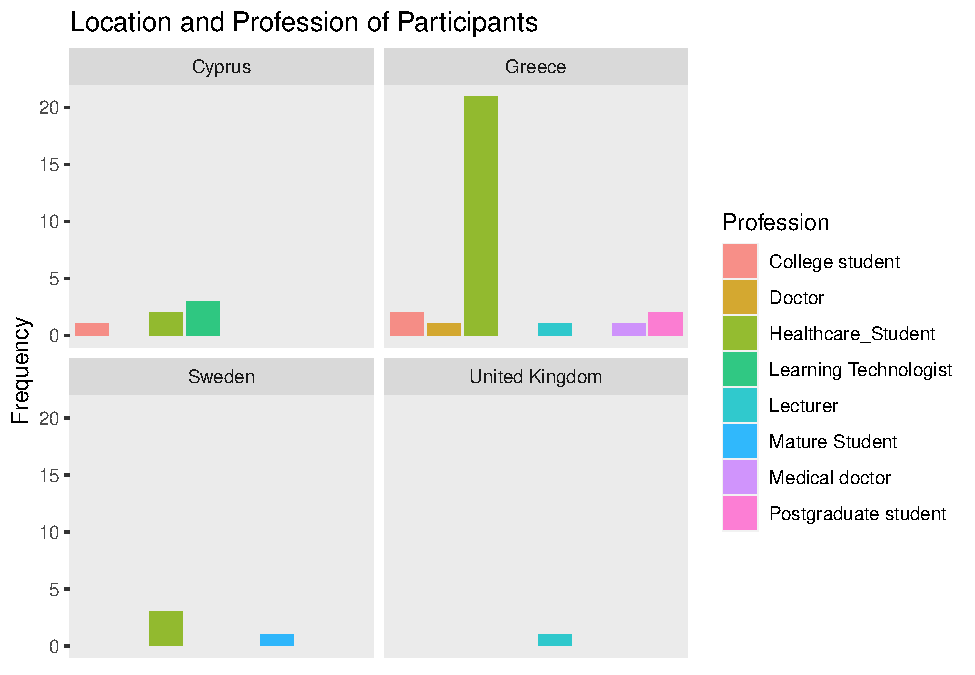
\includegraphics{_main_files/figure-latex/location Boxplotsplits1-1.pdf}

The majority 36 participants, were student, with 3 being learning technologists, 2 were lecturers, and 1 was a doctor.
Although there could be a difference in these groups, the design was within- groups therefore each participants pre-usage metrics were the comparative control data, and participant differences did not affect the evaluation.

\hypertarget{procedure}{%
\section{Procedure}\label{procedure}}

For each resource created by the Partners, the same experimental methodology was followed.
For each resource created by partners, students performed a study within an online or face to face workshop or course.
Student participants joined from Greece, Cyprus, Sweden, and the United Kingdom.
A repeated measures design was used as the same group measures were taken before and after usage of the chatbots.
They were recruited via staff members in the CEPEH group.

Participants were asked prior to the study if they agree to participate, providing them with a PIS form.
Participants had the opportunity to discuss with the research team prior to the study and before consent is given.
Then, participants used the chatbot resources independently and technical support was provided.
Finally, post-intervention measures were recorded.

Some of the participants were invited to participate in Focus Group Discussions (FGD), and each FGD lasted between 15 to 25 minutes, with 5-10 participants.
Participants were asked if they would like to be informed of the findings of the study.

\hypertarget{design}{%
\section{Design}\label{design}}

The data captured from the participants were their initials and numerical day of birth, used as anonymous identifier for pre-post analysis.
Their institution was captured (Aristotle University of Thessaloniki, CYENS Centre of Excellent, Karolinska Institute, and The University of Nottingham), and Sex (Male/Female/Other).

Before any interaction with the learning resources, various perceptions of chatbot such as confidence and easy of use, usefulness, Influence from others, and current learning resources (videos, textbooks, Google, friends etc), were captured.
Descriptive data was produced alongside repeated measures t-tests.
Repeated measures t-tests were the appropriate test to use as this explores differences between groups, there were no covariates and we did not have several dependant variables.
There was one Independent factor being Chatbot use having 2 levels (pre/post).
There were 3 chatbots therefore there was option for ANOVA to determine where differences lie if statistical differences were found however this was not wholly appropriate for the data type and not necessary for pre-post comparison.

\hypertarget{materials-and-measures}{%
\section{Materials and Measures}\label{materials-and-measures}}

The measures used fit within a newly developed Chatbot Evaluation Framework- which takes the best measures of 5 previous frameworks.
Denecke and Warren \hspace{0pt}{[}2{]}\hspace{0pt} derived several quality dimensions and attributes from previous chatbot literature.
They formed six perspectives from their review of articles and mobile health applications.

These six perspectives were: 1) Task-oriented, 2) Artificial intelligence, 3) System quality perspective, 4) Linguistic perspective, 5) UX Perspective, 6) Healthcare quality perspective.

To capture these perspectives, we used several validated materials that can distinguish these elements of the CEPEH chatbots.

\hypertarget{chatbot-usability-questionnaire-cuq}{%
\subsection{Chatbot Usability Questionnaire (CUQ)}\label{chatbot-usability-questionnaire-cuq}}

The Chatbot Usability Questionnaire (CUQ) \hspace{0pt}{[}4{]}\hspace{0pt} is a new questionnaire specifically designed for measuring the usability of chatbots by an interdisciplinary team from the Ulster University.
CUQ can be used alongside the prevalent System Usability Scale Score (SUS) \hspace{0pt}{[}5{]}\hspace{0pt}.
Multiple metrics are more appropriate when measuring usability of chatbots \hspace{0pt}{[}6{]}\hspace{0pt} therefore a combination of two scores can provide an all-inclusive overview.

\hypertarget{utaut2-unified-theory-of-acceptance-and-use-of-technology}{%
\subsection{UTAUT2 (Unified Theory of Acceptance and Use of Technology)}\label{utaut2-unified-theory-of-acceptance-and-use-of-technology}}

The underpinning theory of the UTAUT2 is that there are four key constructs to the intentions of using technology based resources: 1) performance expectancy, 2) effort expectancy, 3) social influence, and 4) enabling conditions.

The TAM and the UTAUT2 have cross over in measuring technology acceptance, however the UTAUT2 has more applied probing questions.
Few studies exist that use technology acceptance theories for the intention to use products that explicitly incorporate AI.
A recent extension of the UTAUT2 model added five (health, convenience comfort, sustainability, safety, security, and personal innovativeness) additional influencing factors to accommodate for AI {[}7{]}.
This can be used for products in either health, household use, or mobility and can help to explain behavioural intention and use behaviour of chatbots.

\hypertarget{system-usability-scale}{%
\subsection{System Usability Scale}\label{system-usability-scale}}

The System Usability Scale (SUS) was used {[}10{]} and is a widely used and adopted usability questionnaire.
It is popular due to its unbiased and agnostic properties, a non proprietary, and quick scale of 10 questions.

\begin{enumerate}
\def\labelenumi{\arabic{enumi}.}
\tightlist
\item
  I think that I would like to use this system frequently.
\item
  I found the system unnecessarily complex.
\item
  I thought the system was easy to use.
\item
  I think that I would need the support of a technical person to be able to use this system.
\item
  I found the various functions in this system were well integrated.
\item
  I thought there was too much inconsistency in this system.
\item
  I would imagine that most people would learn to use this system very quickly.
\item
  I found the system very cumbersome to use.
\item
  I felt very confident using the system.
\item
  I needed to learn a lot of things before I could get going with this system.
\end{enumerate}

The SUS was developed with a scoring system, in which the following should be performed: For each of the odd numbered questions, subtract 1 from the score.
For each of the even numbered questions, subtract their value from 5.
Add up these numbers to find the total score, then multiply this by 2.5.
The result is a score out of 100 and can be compared against a determined average score of 68.
Further, 80.3 or higher is excellent, and 51 or under suggests significant usability problems.

\hypertarget{computer-self-efficacy-scale-tool}{%
\subsection{Computer Self-Efficacy Scale Tool}\label{computer-self-efficacy-scale-tool}}

The 10 question CSEST was based on the 32-item questionnaire by Murphy, Coover, and Owen (1989).
Participants were provided with the facilitator stating 'Imagine you have found a new technology product that you have previously not used.
You believe this product will make your life better.
It doesn't matter specifically what this technology product does, only that it is intended to make your life easier and that you have never used it before.
I could use the new technology\ldots{}

\begin{enumerate}
\def\labelenumi{\arabic{enumi}.}
\tightlist
\item
  If there was no one around to tell me what to do as I go
\item
  If I had never used a product like it before
\item
  If I had only the product manuals for reference
\item
  If I had seen someone else using it before trying it myself
\item
  If I could call someone for help if I got stuck
\item
  If someone else had helped me get started
\item
  If I had a lot of time to complete the job for which the product was provided
\item
  If I had just the built-in help facility for assistance
\item
  If someone showed me how to do it first
\item
  If I had used similar products before this one to do the same job
\end{enumerate}

\hypertarget{technology-acceptance-model-tam}{%
\subsection{Technology Acceptance Model (TAM)}\label{technology-acceptance-model-tam}}

The Technology Acceptance Model (TAM) {[}1{]} was specifically developed with the primary aim of identifying the determinants involved in computer acceptance in general; secondly, to examine a variety of information technology usage behaviours; and thirdly, to provide a parsimonious theoretical explanatory model.
TAM suggests that attitude would be a direct predictor of the intention to use technology, which in turn would predict the actual usage of the technology.
The only modification to the nine sub-scales of the questionnaire consists of applying the items to the context of chatbots.
All the items, except those measuring attitudes, utilize a seven-point Likert scale ranging from ``strongly agree'' to ``strongly disagree'' with a middle neutral point {[}2{]}.

The nine sub-scales of the questionnaire:

• Ease of use of chatbots • Perceived usefulness of chatbots • Intention of use.
• Attitude toward usage of chatbots.
• Perception of personal efficacy to use a chatbot resource.
• Perception of external control toward chatbots.
• Anxiety toward chatbot use.
• Intrinsic motivation to use chatbot resources.
• Perceived costs of chatbots.

\hypertarget{qualitative-measure--focus-group-discussions}{%
\subsection{Qualitative Measure- Focus Group Discussions}\label{qualitative-measure--focus-group-discussions}}

Focus groups are a pervasive means of market research and provides credible acceptance evaluators regarding the penetration that a product or service will have on a target demographic.Focus groups are a form of qualitative research consisting of interviews or structured discussions, in which a group of people are asked about their perceptions, opinions, beliefs, and attitudes towards a product, service, concept, advertisement, idea, or packaging.

Questions are asked in an interactive group setting where participants are free to talk with other group members.During this process, the researcher either takes notes or records the vital points he or she is getting from the group.
Researchers select members of the focus group carefully for effective and authoritative responses.Relevant stakeholders, then, can use the information collected through focus groups to receive insights on a specific product, issue, or topic focus {[}7{]}.

A series of short focus group sessions identified the feasibility of CEPEH resources for formal curricular integration.These sessions, spanning no more than 1-1.5 hours and consisting of no more than 5-7 persons each explored all axes of curricular integration such as accessibility in the classroom, use case scenarios, technology requirements for curricular integration etc.These axes were formalized by the research team, in each evaluation site, to consider the curricular details of each institution.

\includegraphics[width=5.76in]{untitled-1}

Figure 1: Flow diagram of the recruitment process

\hypertarget{rmd-basics}{%
\chapter{Results}\label{rmd-basics}}

\minitoc 

\noindent

\hypertarget{learner-characteristics}{%
\section{Learner Characteristics}\label{learner-characteristics}}

Most learners use books or online books as resources. Of course, they
may use multiple sources however they were asked to note the primary
source. Only 6 stated their primary sources were \emph{Online
videos/interactive materials} which includes such tools as chatbots.

This can be supported when asked the amount of time participants have
used a chatbot- in any form or subject: 23 stated they had never used a
chatbot, being educational or not. 2 individuals had spent what would be
extensive time with usage- these were the Learning Technologist and
Mature Student.Therefore, we can state that the sample used did not regularly use chatbots for their course learning, with 18/42 having used a chatbot at least once for between 0-4 hours of use in total.

The first boxplot here shows learners perceptions of easy of use of mobile appa dn other educational mobile resources

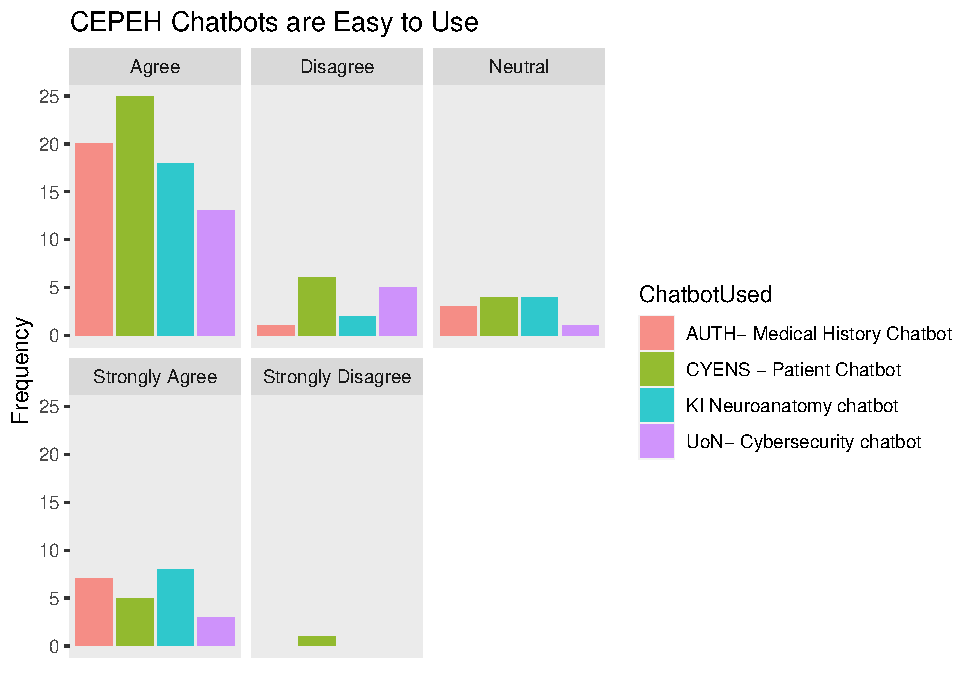
\includegraphics{_main_files/figure-latex/Boxplotsplits3-1.pdf}
There was only 1 `Strongly Disagree' response.
The agreement options counted for the majority of the data.

\begin{longtable}[]{@{}lr@{}}
\toprule()
Previous\_Chatbot\_Usage & n \\
\midrule()
\endhead
1-4 hours & 15 \\
10-19 hours & 1 \\
20+ hours & 1 \\
5-9 hours & 2 \\
Never & 23 \\
\bottomrule()
\end{longtable}

\hypertarget{pre-intervention-results}{%
\section{Pre-Intervention Results}\label{pre-intervention-results}}

\#\#Post-Intervention Results and Comparision

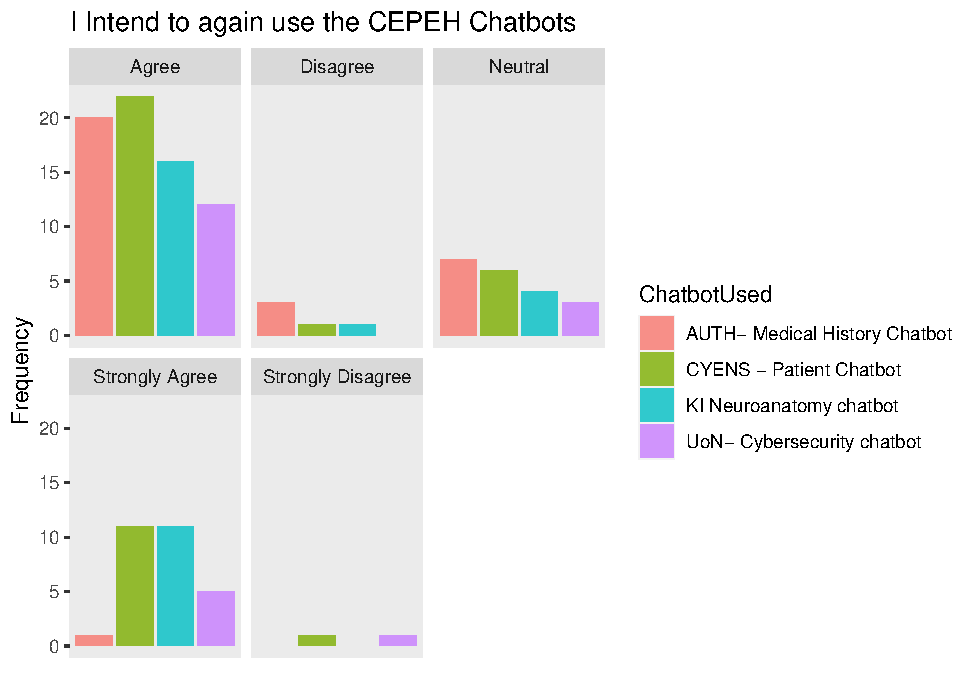
\includegraphics{_main_files/figure-latex/Boxplotsplits4-1.pdf}
For CYENS, even though the knowledge of the topic was not perceived to improve by some participants, this box plot shows how 34/42 stated they would reuse the chatbot developed by CYENS.

\hypertarget{other-findings}{%
\subsection{Other Findings}\label{other-findings}}

Other questions

I intend to continue using chatbots in the future (BI1)
The chatbot provided the information I needed with minimal commands
My knowledge of the topic improved after i had used the Chatbot
My confidence in understanding the topic improved after I had used the
Chatbot
The chatbot provided me with the type of response i expected from asking
a tutor/lecturer
The information provided was reliable
The chatbot has a high level of trustworthiness
The duration of conversations to find my answer was too long
The videos/images provided were useful to my questions
The chatbot exceeded my expectation of how it could help me
The chatbot exceeded my expectation of how it could engage with me
I think this learning method could help me to acquire knowledge
I would use this tool again as it has some value to me
I think i will actively use this learning method
I believe I had some choice about learning during chatbot use
I would trust the chatbot to provide me with information for my course
One piece of knowledge i learned from the chatbot was..

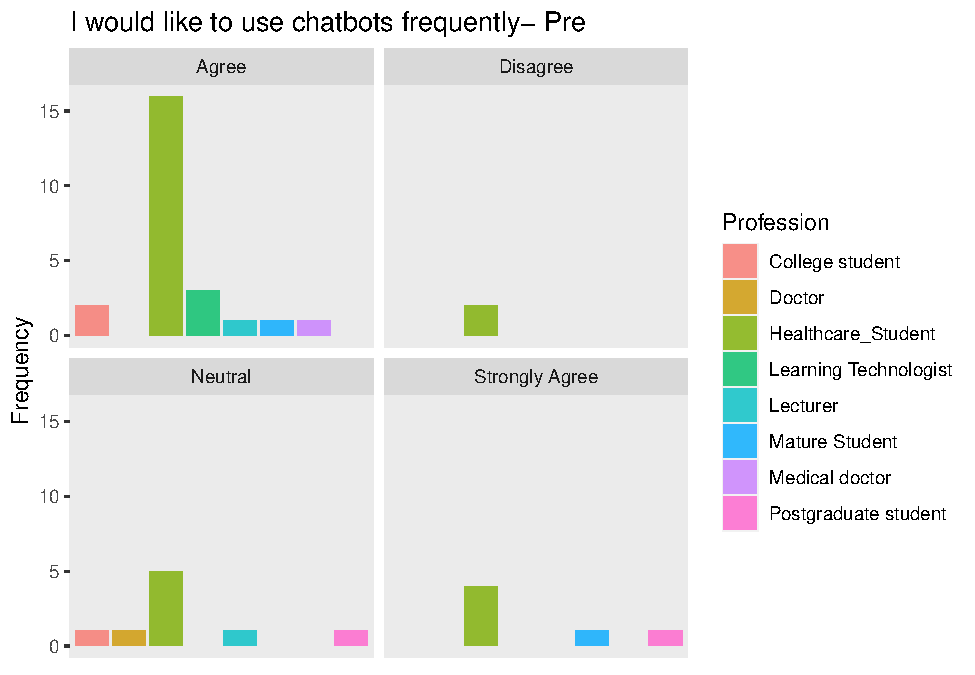
\includegraphics{_main_files/figure-latex/Boxplotsplits2-1.pdf}

Repeated Measures t-test, aka paired t-test (before and after measurements)

This t-test compares confident using mobile chatbots before and after CEPEH chatbot usage.

\hypertarget{system-usability-scale-sus-scores}{%
\subsection{System Usability Scale (SUS) Scores}\label{system-usability-scale-sus-scores}}

\emph{Note= The amount of `agreement' is defined as the addition of `Agree'
and `Strongly agree' responses.}

The SUS score should consist of 10 items. However, some SUS questions
were improved upon by 1 or more CUQ questions, specifically to this
Chatbot study. The SUS results would be overshadowed by the CUQ scores,
expect 2 that did not have cross-over. The two questions were:

\begin{itemize}
\tightlist
\item
  I would like to use the CEPEH chatbot I tested, more frequently
  (SUS1)(post)
\item
  I felt confident using the CEPEH chatbot (SUS2)(post)
\end{itemize}

This meant the score of the SUS was not created, however the CUQ score
better represented the Learners' perceptions of the CEPEH chatbot in
terms of feasibility of reuse and acceptability in healthcare curricula.

\begin{longtable}[]{@{}llr@{}}
\toprule()
Keep\_Using\_Chatbots & Confident & Count \\
\midrule()
\endhead
Agree & Agree & 44 \\
Agree & Disagree & 5 \\
Agree & Neutral & 11 \\
Agree & Strongly Agree & 6 \\
Disagree & Agree & 6 \\
Disagree & Disagree & 5 \\
Disagree & Neutral & 4 \\
Neutral & Agree & 10 \\
Neutral & Disagree & 1 \\
Neutral & Neutral & 6 \\
Not Applicable & Not Applicable & 3 \\
Strongly Agree & Agree & 10 \\
Strongly Agree & Not Applicable & 1 \\
Strongly Agree & Strongly Agree & 12 \\
Strongly Disagree & Agree & 1 \\
Strongly Disagree & Strongly Agree & 1 \\
\bottomrule()
\end{longtable}

\hypertarget{technology-acceptance-model}{%
\subsection{Technology Acceptance Model}\label{technology-acceptance-model}}

The TAM had 3 sections (Ease of Use, Perceived Usefulness, and Intention
of Use). Ease of Use results showed significant increases in Users'
usage with each Chatbot. Perceived Usefulness: There were not
significant findings for the Perceived usefulness. The justification for
this may be due to being early versions of applications with limited
functionality and functions which can be difficult for user to
experience the intended further range of features and learning
exercises.

Intention of Use: For users' intentions to use within their course, the
result of the Mann-Whitney U test was not significant, U = , z = , p = .
in their intentions before use (m=xx, mode=xx) compared to after (m=xx,
mode=x), however there was improvement therefore the chatbots may have
more benefit than expected by students.

\hypertarget{chatbot-usabilty-questionanire-cuq}{%
\section{Chatbot Usabilty Questionanire (CUQ)}\label{chatbot-usabilty-questionanire-cuq}}

\hypertarget{cuq-calcuation-tool}{%
\subsection{CUQ Calcuation tool}\label{cuq-calcuation-tool}}

The CUQ was developed by researchers at Ulster University,\href{\%3Ca\%20href=\%22https://www.ulster.ac.uk/research/topic/computer-science/artificial-intelligence/projects/cuq\%22}{Link}
and as the calculation can be complex a dedicated calculation tool has been created.
Please download the CEPEH CUQ calculation tool which has all of the data entered, so you can see the CEPEH CUQ scoring.

\href{CUQ-Calculation-Tool.xlsx}{click here to download CUQ calc tool}

\href{cuq.png}{click here to download CUQ score image}
*mobile download disabled

\begin{figure}

{\centering 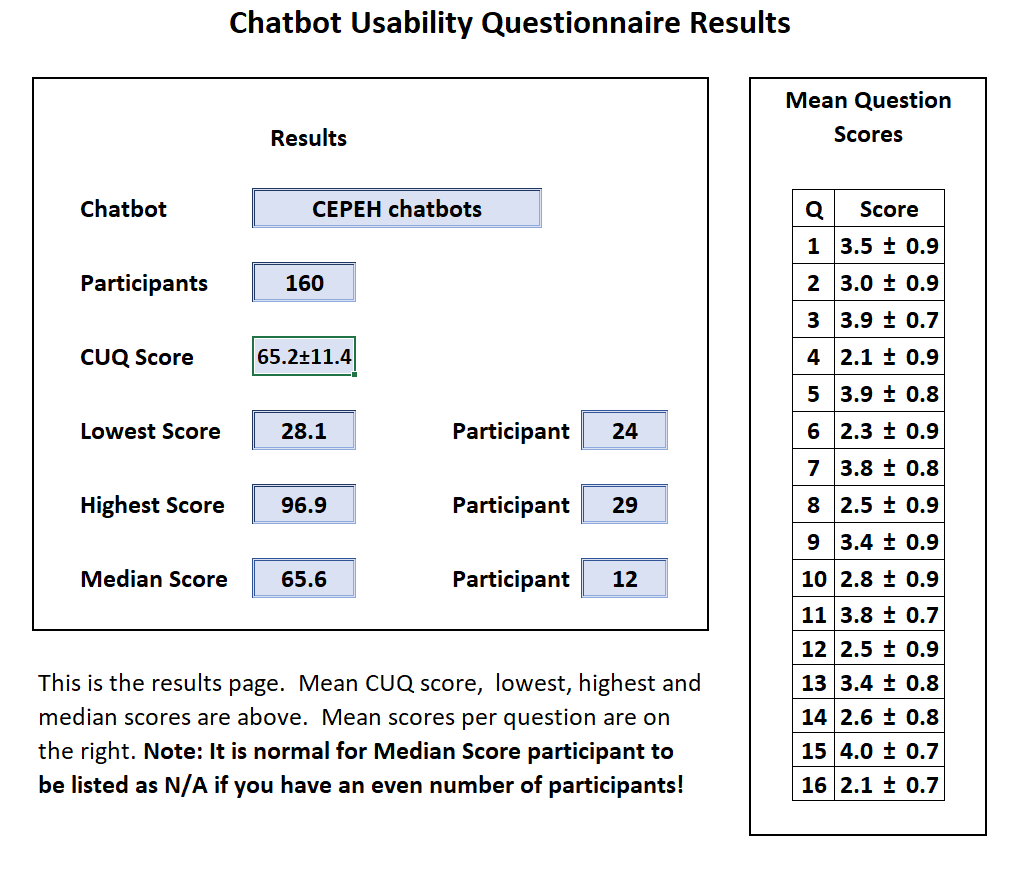
\includegraphics[width=0.75\linewidth]{cuq} 

}

\caption{A marvel-lous meme}(\#fig:cuq image)
\end{figure}

The score for all 3 chatbots grouped was 65.2/100,
This scoring system was designed to be comparable to SUS and may be
freely used alongside it, or in combination with other usability
metrics. There has been evidence of correlation of 76\% between the CUQ
and SUS therefore we expect the SUS scored to be between 48.75 and 81\%.
We believe the CUQ has more validity towards measuring the concepts of
interest on this study.

\href{\%3Ca\%20href=\%22https://dl.acm.org/doi/pdf/10.1145/3335082.3335094?casa_token=rGs2gNvKuLkAAAAA:Cd8Qn3QywYHZGYJzbD5CU1dVFWHPLGzDnmQYue6ix-AcqOkWLa7VN4GuzvfrZR2DhhvEAoZOF_2T}{Read the CUQ development paper, see page 3 for correlation}

Figure shows the CUQ scores as a box plot to highlight the range of Usability of the resources. Further exploration is required to understand which elements are causing this spread.

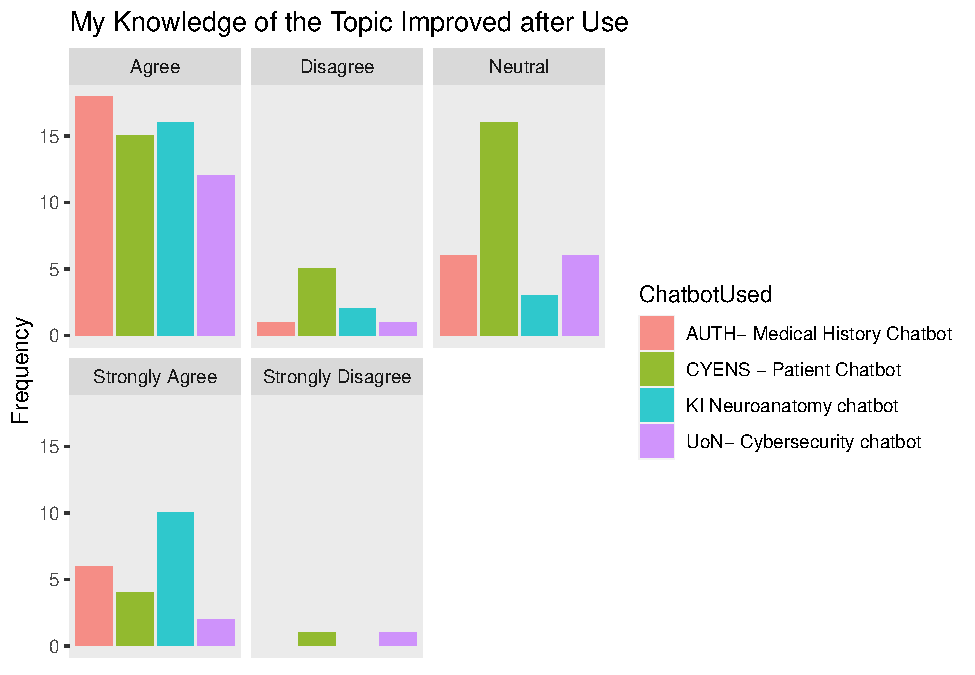
\includegraphics{_main_files/figure-latex/Boxplotsplits5-1.pdf}
CYENS chatbot had around 10 more participants stating that they were neutral on gaining knowledge of the topic

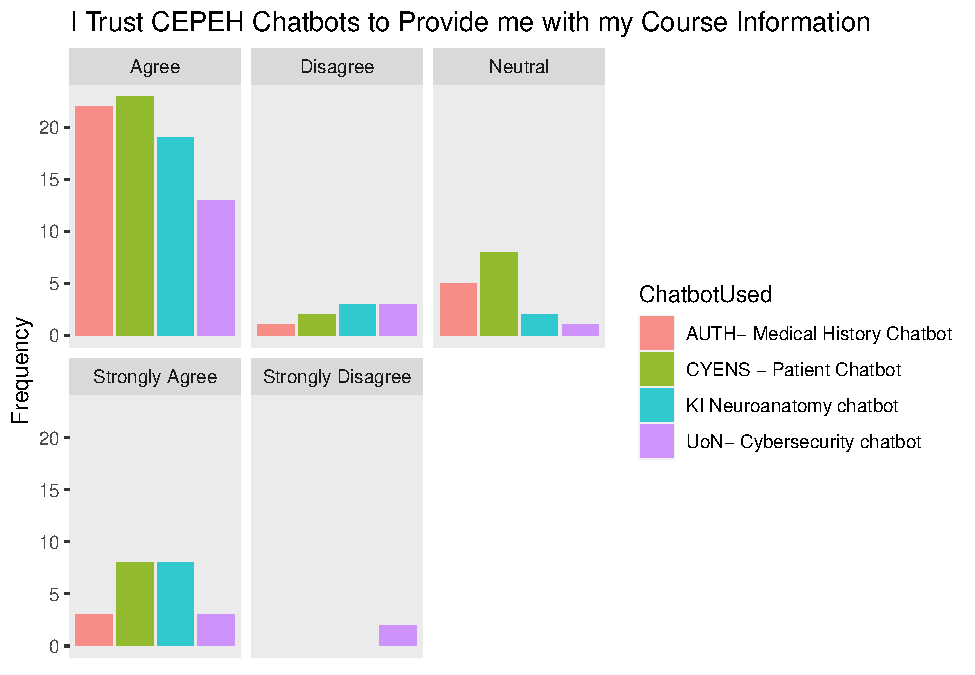
\includegraphics{_main_files/figure-latex/Boxplotsplits6-1.pdf}

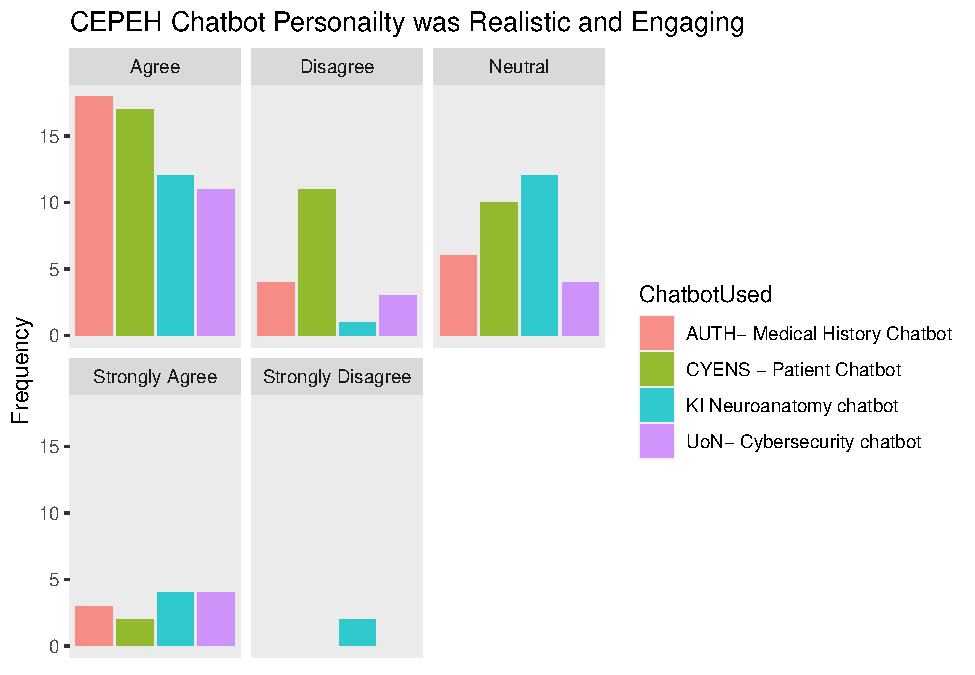
\includegraphics{_main_files/figure-latex/Boxplotsplits7-1.pdf}
There was mixed results for the chatbot used being realistic and engaging. This question has two descriptive terms however based on the other results we understand that the chatbots' NLP logic, or ability to respond required improvement to be more `smooth' in replying. The primary limitation was found in the `robotic' interactions(See Figure 10). This was investigated further in the `Text Mining' and `Sentiment Analysis' sections.

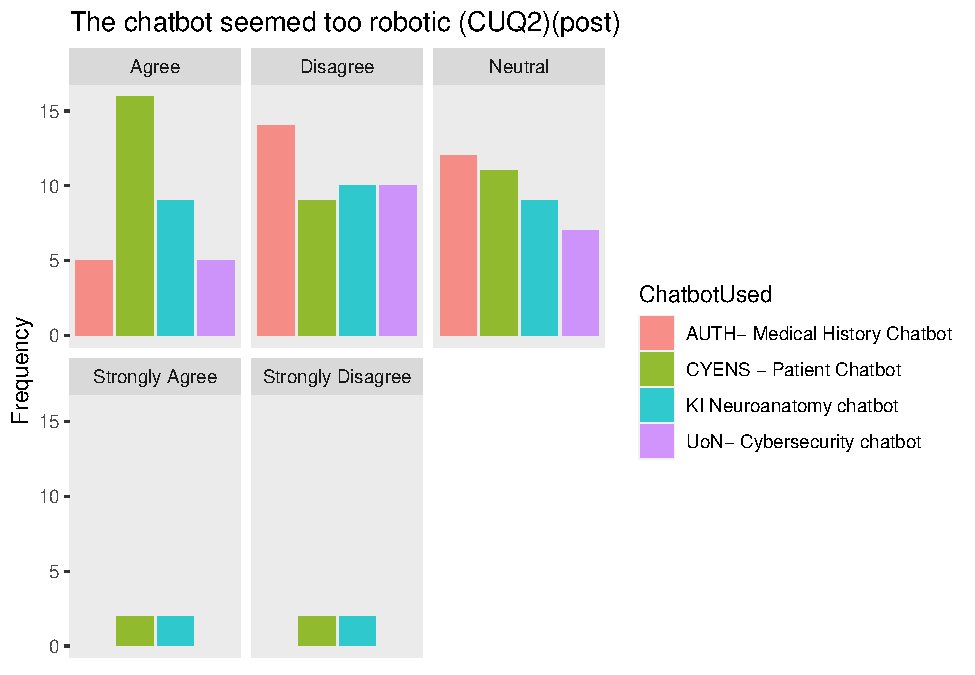
\includegraphics{_main_files/figure-latex/Boxplotsplits8-1.pdf}

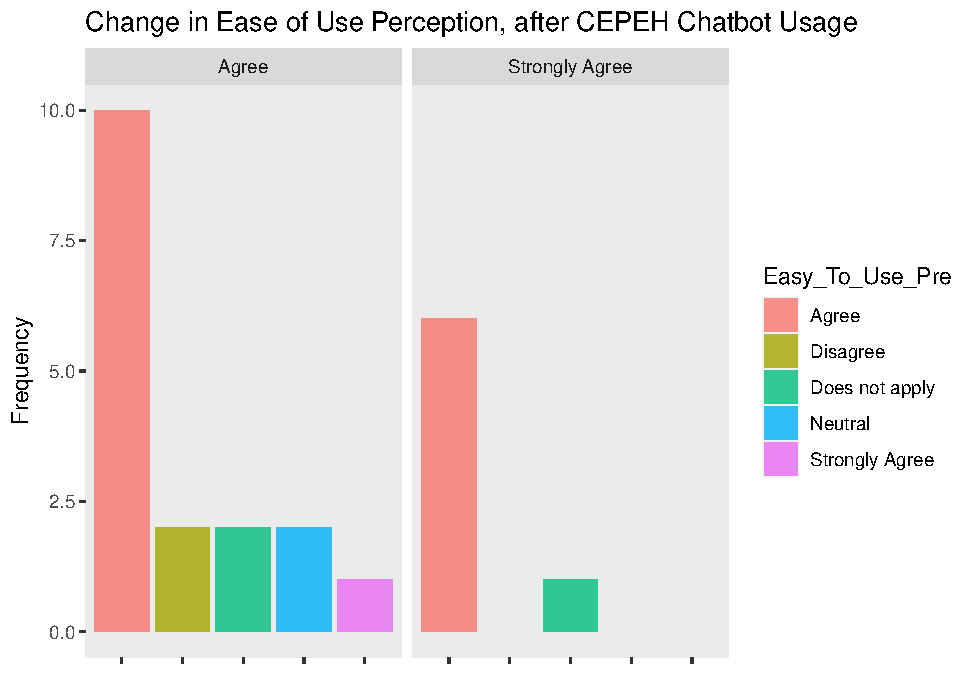
\includegraphics{_main_files/figure-latex/Boxplotsplits9-1.pdf}

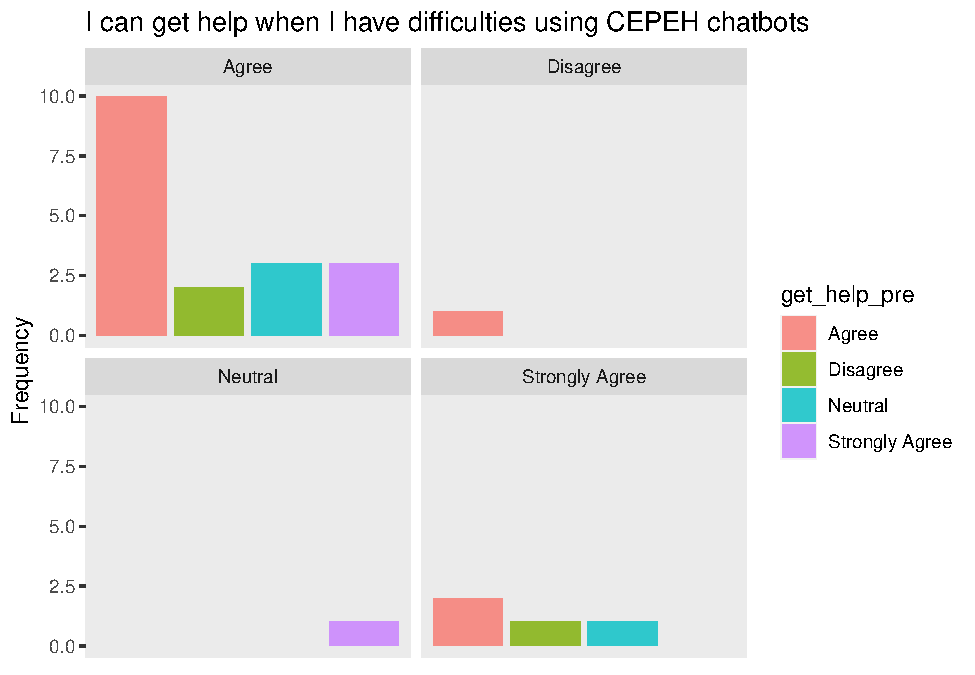
\includegraphics{_main_files/figure-latex/Boxplotsplits10-1.pdf}
Those who disagreed or were neutral in the pre usage measure, improved their understanding that help was available
with the CEPEH chatbots. After usage, 40 participants agreed they could get help if they had difficulty using the
resources.

\hypertarget{inferential-statistics}{%
\section{Inferential Statistics}\label{inferential-statistics}}

output:
\#bookdown::html\_document2: default
\#bookdown::word\_document2: default
bookdown::pdf\_document2:
template: templates/template.tex
documentclass: book

\#bibliography: {[}bibliography/references.bib, bibliography/additional-references.bib{]}

\hypertarget{text-mining-natural-language-processing-and-sentiment-analysis}{%
\chapter{Text Mining, Natural Language Processing, and Sentiment Analysis}\label{text-mining-natural-language-processing-and-sentiment-analysis}}

\hypertarget{cepeh-qualatative-feedback}{%
\section{CEPEH Qualatative Feedback}\label{cepeh-qualatative-feedback}}

The focus group discussions provided a lot of feedback for how the participants experienced their interactions with the chatbots, and how the CEPEH team can improve them, improve the design and development processes, and improve uptake and sharing.

One method of analysing this data is with use of text mining and data manipulation, creating word clouds, sentiment analysis, and using a model which can distinguish the unique themes in text, and highlights for us what text is used to create these themes.

Therefore, we have created a model to allow efficient and intelligent analysis of this open/free focus group data.

\hypertarget{tokenising}{%
\section{Tokenising}\label{tokenising}}

Firstly, we tokenised the words from the FGDs. A Token is ``a meaningful unit of text, most often a word, that we are interested in using for further analysis''. For each word we give it a property that we can call upon later.

The data manipulation for this included removing punctuation, converting to lower-case, and setting word type to word (and not such types as ``characters'', ``ngrams'', ``sentences'', ``lines'' etc)

\hypertarget{stop-words}{%
\subsection{Stop words}\label{stop-words}}

The model then removed words with meaningless function. These are called stop words. Words like ``the'', ``of'' and ``to'' are the most frequent words found, technically, but are of little interest to us.

We also created a custom list of stop words for CEPEH. We know participants may mention other objects, and the list was as followed: found; chatbot; chatbots; presentation.

The data was ready for analysis by the model. We ordered it to find the most frequent words.

\hypertarget{plotting-word-frequencies---bar-graphs}{%
\section{Plotting word frequencies - bar graphs}\label{plotting-word-frequencies---bar-graphs}}

With this information a Bar graph of top words from the participants in the FGD can be rendered.

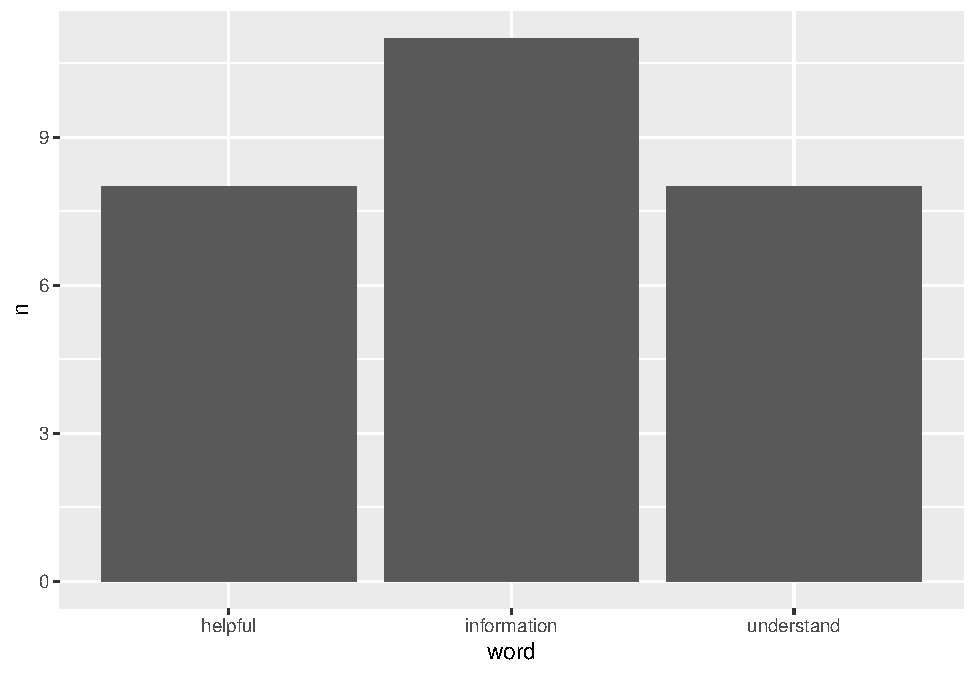
\includegraphics{_main_files/figure-latex/FREQ words bar graph-1.pdf}

and after some modifications, a graph of the top 35 words is produced, with better aesthetics.The most frequent words present in focus group discussions after using the 4 chatbots, are in the Figure below.

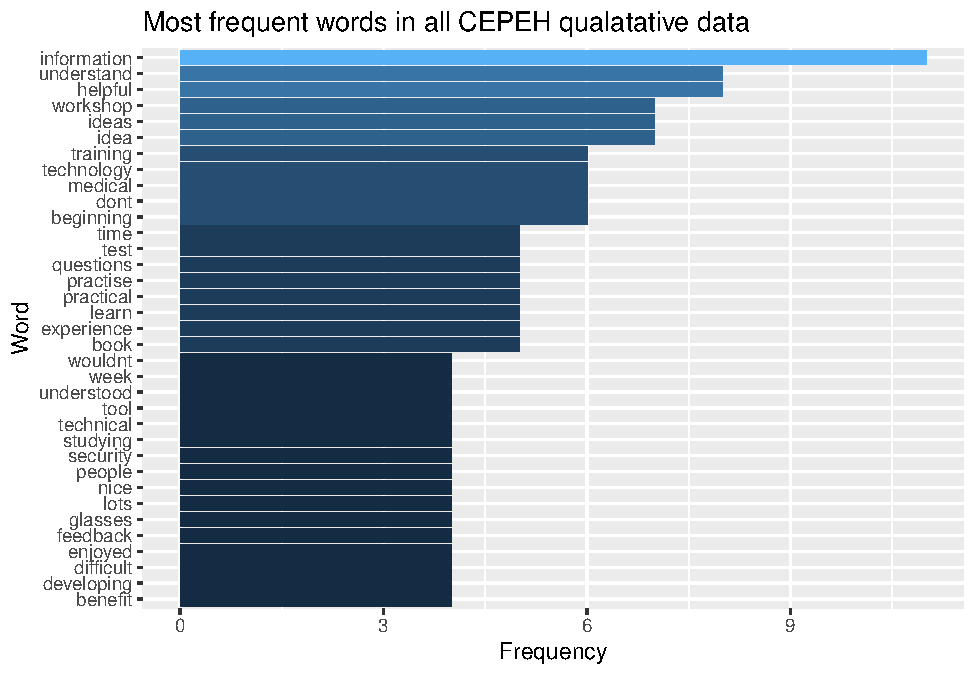
\includegraphics{_main_files/figure-latex/unnamed-chunk-8-1.pdf}

Although the frequency is not high for each word, we are able to get a general picture of the sentiments, intensities, and concerns which would be immediately occurring when plotted.

\hypertarget{normalised-frequency}{%
\subsection{Normalised frequency}\label{normalised-frequency}}

A better way to understand this data is to normalise the frequency of occurrences in accordance with the source text. The raw text had 2827 words in total. Therefore we can mutate the ratios to reflect this.

\hypertarget{plotting-normalised-frequency}{%
\subsubsection{Plotting normalised frequency}\label{plotting-normalised-frequency}}

Now we can plot, for example, the 20 most frequent words when normalised by the source text.

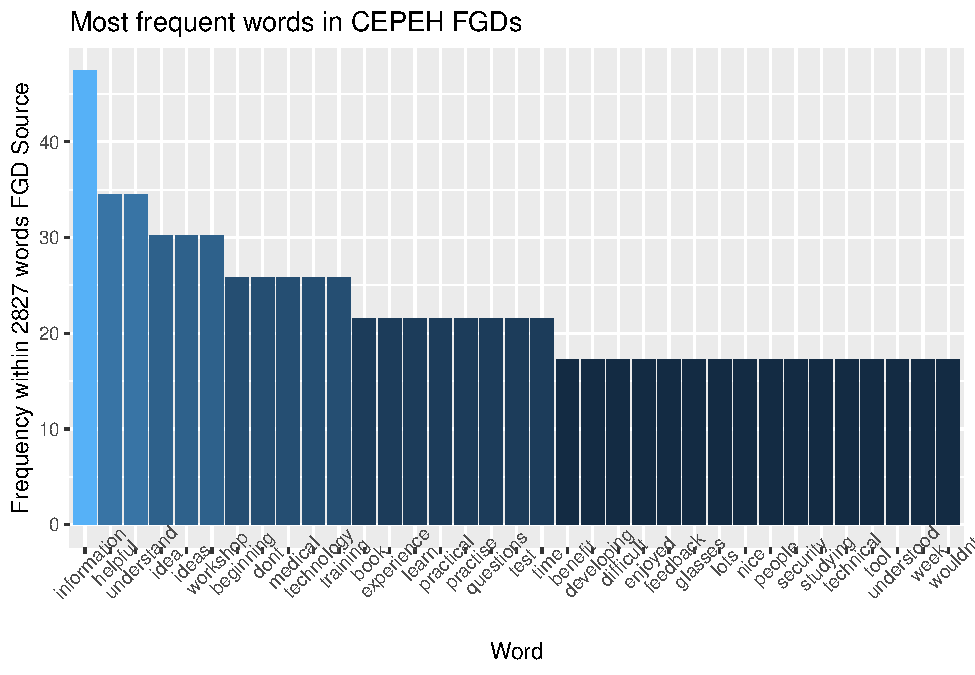
\includegraphics{_main_files/figure-latex/CEPEH MOST FREQ-1.pdf}
In summary, this understanding of frequent words can help to understand common concurrences and extrapolate to a larger audience. If scope and impact of CEPEH chatbots increased we can understand the type of themes and trends may occur, based on such FGD analysis.

\hypertarget{word-clouds}{%
\section{Word clouds}\label{word-clouds}}

To visualise the most frequent words in another format, below is a word cloud which presents the word size to indicate the frequency- words that occur more often being displayed in a larger font size.
This has a normalised data frequency in accordance to the FGD source document analysed.

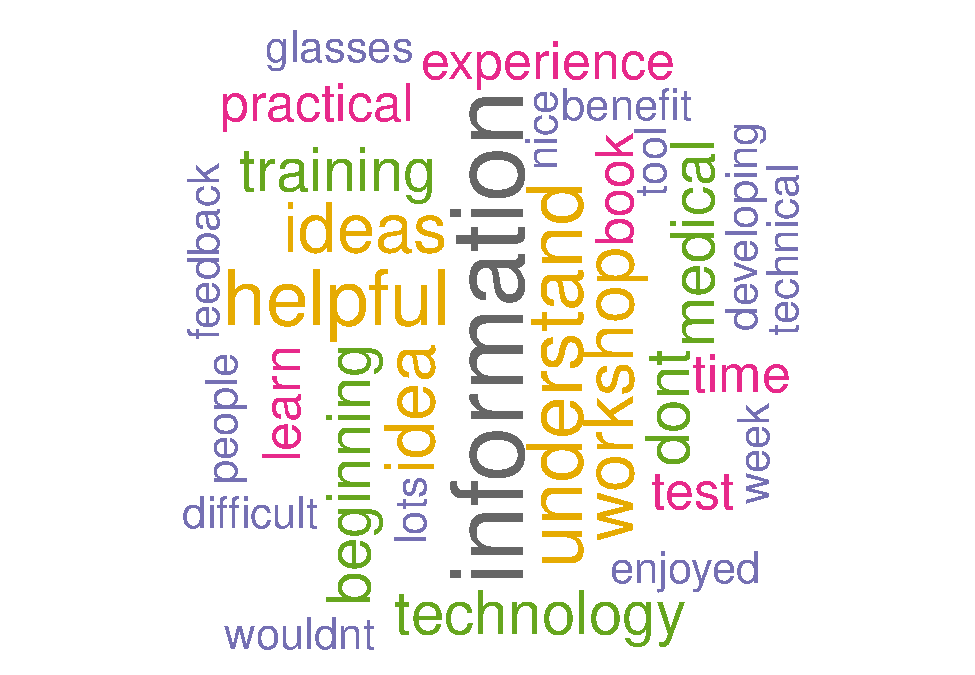
\includegraphics{_main_files/figure-latex/unnamed-chunk-10-1.pdf}
We understand the context has been reduced for each word. However, in general there can be categorised positive/negative words from the word cloud:
Positive words are- benefit, practical, nice, helpful, learn, ideas, and enjoyed
Negative words are- difficult, test (who likes a test?), don't, and `lot' may be negative if there is a `lot' of information.

\hypertarget{the-vocabulary-of-texts}{%
\subsection{The vocabulary of Texts}\label{the-vocabulary-of-texts}}

Here is a graph that has plotted the words in places depending on the word frequencies. Additionally, colour hotspots shows how different the frequencies are - darker items are more similar in terms of their frequencies, lighter-coloured ones more frequent in one text compared to the other.
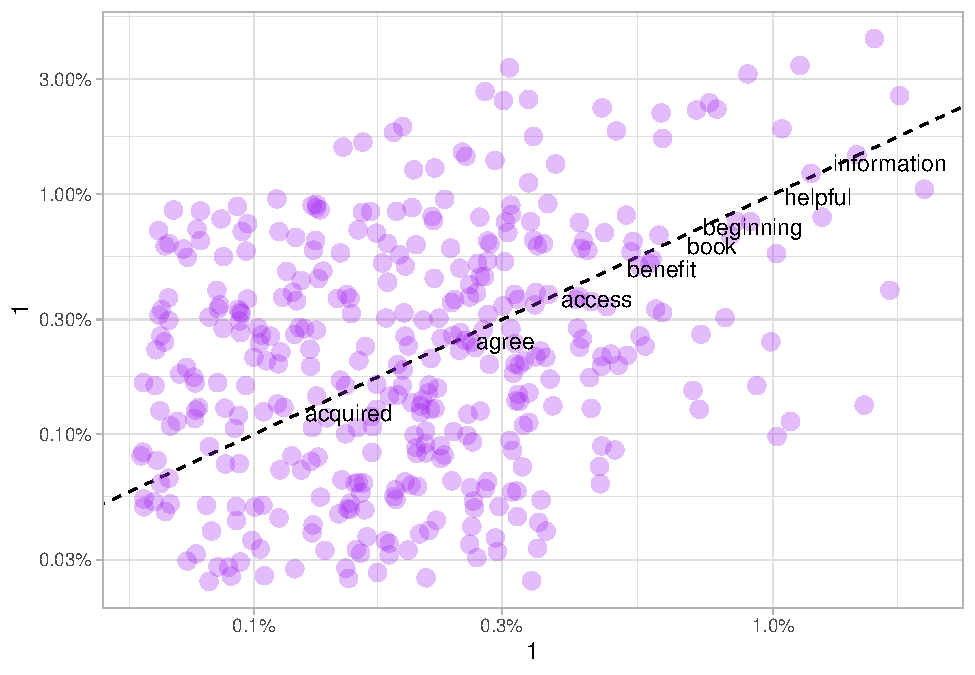
\includegraphics{_main_files/figure-latex/unnamed-chunk-12-1.pdf}

\hypertarget{sentiment-analysis}{%
\section{Sentiment analysis}\label{sentiment-analysis}}

What is the sentiment of all participants? What is types of emotional words are being used?
The preparation of these words has some use in understanding the frequencies, but their emotional valence are not compared. The table above has the word \emph{`helpful'} which has a positive connotation, however there are 386 words, with many having several occurrences.

\begin{verbatim}
##   max(total_score) min(total_score)
## 1               38               38
\end{verbatim}

\begin{tabular}{r|r|r}
\hline
negative & positive & total\_score\\
\hline
24 & 62 & 38\\
\hline
\end{tabular}

\begin{verbatim}
output:
  #bookdown::html_document2: default
  #bookdown::word_document2: default
  bookdown::pdf_document2:
    template: templates/template.tex
    keep_tex: true

#bibliography: [bibliography/references.bib, bibliography/additional-references.bib]

  bookdown::html_document2: default
  bookdown::word_document2: default
documentclass: book
\end{verbatim}

\begin{center}\rule{0.5\linewidth}{0.5pt}\end{center}

\hypertarget{Discussion}{%
\chapter{Discussion}\label{Discussion}}

\minitoc 

The Chatbots were beneficial.

Learners have lots of other choices such as YouTube, but there is a certain need for personalised information gathering , this can save time and prevent learning incorrect information.

This was one reason why they were rated positive as they are able to streamline data finding for learners in a format that is understandable and easy to them.

\begin{tabular}{llllllllllllllllllllllllllllllllllllllllllllllllllllllllllllllllllllllllllllllllllr}
\toprule
sex & time & Code & Location & Profession & CurrentMaterials & Previous\_Chatbot\_Usage & UseChatbotsFrequently & I feel very confident using mobile apps (pre) & UsefulPE1PRE & IncreaseAchievingPE2PRE & AccomplishThingsQuicklyPE3PRE & IncreasesProductivityPE4PRE & HowToUse(EE1)(pre) & InteractionsClearUnderstandable(EE2)(pre) & EasyToUse(EE3)(pre) & EasySkilfulUsing(EE4)(pre) & PeopleImportantUse(SI1)(pre) & PeopleInfluenceUse(SI2)(pre) & PeopleOpinionsUse(SI3)(pre) & ResourcesNecessary(FC1)(pre) & KnowledgeNecessary(FC2)(pre) & CompatibleOtherTech(FC3)(pre) & GetHelpWhenDifficuly(FC3)(pre) & Enjoyable(HM2)(pre) & Entertaining(HM3)(pre) & ContinueUsing(BI1)(pre) & ChatbotUsed & The chatbot provided the information I needed with minimal commands(post) & My knowledge of the topic improved after i had used the Chatbot(post) & My confidence in understanding the topic improved after I had used the Chatbot(post) & The chatbot provided me with the type of response i expected from asking a tutor/lecturer(post) & The information provided was reliable (post) & The chatbot’s personality was realistic and engaging (CUQ1)(post) & The chatbot seemed too robotic (CUQ2)(post) & The chatbot was welcoming during initial setup (CUQ3)(post) & The chatbot seemed very unfriendly (CUQ4)(post) & The chatbot explained its scope and purpose well (CUQ5)(post) & The chatbot gave no indication as to its purpose (CUQ6)(post) & The chatbot was easy to navigate (CUQ7)(post) & It would be easy to get confused when using the chatbot (CUQ8)(post) & The chatbot understood me well (CUQ9)(post) & The chatbot failed to recognise a lot of my inputs (CUQ10)(post) & Chatbot responses were useful, appropriate and informative (CUQ11)(post) & Chatbot responses were irrelevant (CUQ12)(post) & The chatbot coped well with any errors or mistakes (CUQ13)(post) & The chatbot seemed unable to handle any errors (CUQ14)(post) & The chatbot was very easy to use (CUQ15)(post) & The chatbot was very complex (CUQ16)(post) & I would like to use the CEPEH chatbot i tested, more frequently (SUS1)(post) & I felt confident using the CEPEH chatbot (SUS2)(post) & The chatbot has a high level of trustworthiness(post) & The duration of conversations to find my answer was too long(post) & I found the CEPEH chatbots useful in my daily life (PE1)(post) & Using CEPEH chatbots increases my chances of achieving things important to me (PE2)(post) & Using CEPEH chatbots can help me accomplish things more quickly (PE3)(post) & Using CEPEH chatbots increases my productivity (PE4)(post) & Learning how to use CEPEH chatbots is easy for me (EE1)(post) & My interaction with CEPEH chatbots is clear and understandable (EE2)(post) & I find CEPEH chatbots easy to use (EE3)(post) & It is easy for me to become skilful at using CEPEH chatbots (EE4)(post) & People who are important to me think that I should use CEPEH chatbots (SI1)(post) & People who influence my behaviour think that I should use CEPEH chatbots (SI2)(post) & People whose opinions that I value prefer that I use CEPEH chatbots (SI3)(post) & I have the resources necessary to use CEPEH chatbots (FC1)(post) & I have the knowledge necessary to use CEPEH chatbots (FC2)(post) & CEPEH Chatbots are compatible with other technologies I use (FC3)(post) & I can get help from others when I have difficulties using CEPEH chatbots (FC4)(post) & Using CEPEH chatbots is enjoyable (HM2)(post) & Intend & The videos/images provided were useful to my questions(post) & The chatbot exceeded my expectation of how it could help me(post) & The chatbot exceeded my expectation of how it could engage with me(post) & The chatbot exceeded my expectation of how entertaining it was to use(post) & I think this learning method could help me to acquire knowledge(post) & Reuse & I think i will actively use this learning method(post) & I believe i had some choice about learning during chatbot use(post) & I would trust the chatbot to provide me with information for my course(post) & One piece of knowledge i learned from the chatbot was..(post) & Informed of results(post) & Date (post) & CUQ\\
\midrule
Female & Pre & 666 & Cyprus & Student on a Healthcare course & Books & Never & Agree & Strongly Agree & Agree & Agree & Agree & Agree & Agree & Neutral & Agree & Agree & Neutral & Neutral & Neutral & Neutral & Neutral & Agree & Agree & Agree & Agree & Agree & NA & NA & NA & NA & NA & NA & NA & NA & NA & NA & NA & NA & NA & NA & NA & NA & NA & NA & NA & NA & NA & NA & NA & NA & NA & NA & NA & NA & NA & NA & NA & NA & NA & NA & NA & NA & NA & NA & NA & NA & NA & NA & NA & NA & NA & NA & NA & NA & NA & NA & NA & NA & NA & NA & NA & 56.2500\\
NA & Post & 666 & NA & NA & NA & NA & NA & NA & NA & NA & NA & NA & NA & NA & NA & NA & NA & NA & NA & NA & NA & NA & NA & NA & NA & NA & CYENS - Patient Chatbot & Disagree & Neutral & Neutral & Neutral & Agree & Neutral & Agree & Agree & Neutral & Disagree & Agree & Neutral & Neutral & Disagree & Agree & Neutral & Neutral & Disagree & Neutral & Disagree & Neutral & Neutral & Neutral & Neutral & Agree & Neutral & Disagree & Neutral & Neutral & Neutral & Neutral & Neutral & Neutral & Agree & Agree & Agree & Agree & Neutral & Disagree & Agree & Neutral & Neutral & Neutral & Disagree & Neutral & Neutral & Neutral & Neutral & Neutral & Agree & Agree & Medical scenarios & YES & 2022-05-11 08:14:34 UTC & 68.7500\\
Male & Pre & A.S.1507 & Greece & Student on a Healthcare course & Online journals\_books & Never & Neutral & Agree & Neutral & Neutral & Agree & Neutral & Agree & Agree & Agree & Agree & Neutral & Neutral & Neutral & Agree & Disagree & Agree & Disagree & Agree & Agree & Agree & NA & NA & NA & NA & NA & NA & NA & NA & NA & NA & NA & NA & NA & NA & NA & NA & NA & NA & NA & NA & NA & NA & NA & NA & NA & NA & NA & NA & NA & NA & NA & NA & NA & NA & NA & NA & NA & NA & NA & NA & NA & NA & NA & NA & NA & NA & NA & NA & NA & NA & NA & NA & NA & NA & NA & 64.0625\\
NA & Post & A.N. 31082003 & NA & NA & NA & NA & NA & NA & NA & NA & NA & NA & NA & NA & NA & NA & NA & NA & NA & NA & NA & NA & NA & NA & NA & NA & NA & NA & NA & NA & NA & NA & NA & NA & NA & NA & NA & NA & NA & NA & NA & NA & NA & NA & NA & NA & NA & NA & NA & NA & NA & NA & NA & NA & NA & NA & NA & NA & NA & NA & NA & NA & NA & NA & NA & NA & NA & NA & NA & NA & NA & NA & NA & NA & NA & NA & NA & NA & NA & NA & NA & 51.5625\\
NA & Post & A.N. 31082003 & NA & NA & NA & NA & NA & NA & NA & NA & NA & NA & NA & NA & NA & NA & NA & NA & NA & NA & NA & NA & NA & NA & NA & NA & NA & NA & NA & NA & NA & NA & NA & NA & NA & NA & NA & NA & NA & NA & NA & NA & NA & NA & NA & NA & NA & NA & NA & NA & NA & NA & NA & NA & NA & NA & NA & NA & NA & NA & NA & NA & NA & NA & NA & NA & NA & NA & NA & NA & NA & NA & NA & NA & NA & NA & NA & NA & NA & NA & NA & 84.3750\\
\addlinespace
Female & Pre & AG 26062002 & Greece & Student on a Healthcare course & Books & Never & Agree & Neutral & Agree & Neutral & Neutral & Agree & Agree & Neutral & Neutral & Neutral & Neutral & Neutral & Neutral & Agree & Neutral & Agree & Agree & Agree & Agree & Agree & NA & NA & NA & NA & NA & NA & NA & NA & NA & NA & NA & NA & NA & NA & NA & NA & NA & NA & NA & NA & NA & NA & NA & NA & NA & NA & NA & NA & NA & NA & NA & NA & NA & NA & NA & NA & NA & NA & NA & NA & NA & NA & NA & NA & NA & NA & NA & NA & NA & NA & NA & NA & NA & NA & NA & 76.5625\\
\bottomrule
\end{tabular}

\hypertarget{cites-and-refs}{%
\chapter{Training Event Results}\label{cites-and-refs}}

\chaptermark{Citations and cross-refs}

\minitoc 

\hypertarget{cepeh-training-event-c1}{%
\section{CEPEH Training Event C1}\label{cepeh-training-event-c1}}

The CEPEH training event C1 held at the premises of University of Nottingham aiming to prepare participants for the practical elements of co-creation and implementation of chatbots as an educational resource. It combined both theoretical and hands-on training.
15 participants were from RISE, AUTH, UoN.

Project managers of partners signposted the person involved, and relevant announcements were made though social media channels to the wider public. External to the project speakers were from University of Leeds, and Computer Science Department of University of Nottingham. It included academics, medical doctors, and researchers with focus both on clinical research and digital innovations in healthcare education and IT specialist/learning technologists 11.18 years of experiences (SD=7.2). A balance between male and female participants achieved.

\hypertarget{overall-training-events-evalaution}{%
\chapter{Overall Training Events Evalaution}\label{overall-training-events-evalaution}}

Participants were asked to highlight what they liked for each day and how each day can be improved. Findings are described below per day of the training event

Day 1\\
The participants comment that they liked the design method for educational resources presented using a co-creation approach, they liked the interactions with other groups, and they liked the overview of existing chatbot resources of the partners. On the areas that can be improved, more media material were requested.

Day 2
Participants enjoyed the presentation from the invited speaker from another faculty of the University of Nottingham, the CEPEH recources presented and the storyboarding process. Participants highlighted that the participation of more clinicians in the event would be an added value in regards with the storyboarding process.

Day3
Participants liked the hands-on activities of the day also enjoyed the creativity of the groups on the online chatbot development tool. As an area of improvement, participants wanted more time on hands on sections.

\hypertarget{cepeh-training-event-2}{%
\section{CEPEH Training Event 2}\label{cepeh-training-event-2}}

\textbf{Pre-Training Event survey May 9th-13th 2022 Thessaloniki, Greece}

Twenty-six participants attended the Training Event, along with approximately 10 staff members. There were 21 undergraduate students and 5 postgraduate students, who completed the survey for a total of 26 responses. There were 86\% of participants who stated they had not been to a similar event like the training event CEPEH facilitated. There were 90\% of students who found the event schedule very organised, and 70\% agreed most of the planned sessions were relevant to that interest with the remaining 30\% not having enough experience to understand the context to determine if they are interested in the training event. There were 95\% of students agreeing or strongly agreeing the training event location is great, the remaining person did not leave additional comments.

Table 1 suggested attendees had minimal intention to share their own ideas due to lack of previous experience of attending such events, or due to lack of knowledge on the area. However, most were interested in listening to other groups and hearing contextual cases in healthcare.

There were 77\% of participants stated they were novices in experience with chatbots in healthcare and were attending to learn more. The remaining 23\% (7 students) stated they were competent and had limited experience with chatbots in healthcare.

One day had several events regarding cybersecurity in healthcare. When asked before these events, 83\% stated they were neutral or disagreed that they felt confident about their cybersecurity knowledge in healthcare. In addition, 80\% stated they when neutral or disagreed that they felt they had strong cybersecurity safety in healthcare. Table 2 shows the main pre and post results suggesting a positive experience for more than 75\% of attendees on all measures.

There were 90\% (23) of students who heard about the event through a lecturer or a professor, the CEPEH newsletter (2), and 1 person was informed through the anatomy tutoring system at Karolinska Institute. Additionally, 60\% suggested the training event to somebody else before the course started.

There were six individuals who stated neutral or disagree when asked if having issues on registration or finding the information for the event. This may have been due to being dependent on emails to receive the information, instead of a dedicated website where the information is available anytime.

As this was face-to-face, participants were asked about sufficient Covid-19 precautions in place at the facility, 94\% agreed with sufficient precautions, two individuals stated no but did not give further information in the additional input box provided.
In summary, most participants were undergraduate students with novice experience, happy with the training event location, felt the sessions were relevant to them, and most shared the event with their colleagues. The values of co-creation, chatbots in healthcare, and taking patient history were bestowed to students in an engaging and well-received manner. Notably, the highest ratings were for staff friendliness which is key to engagement and consistent interaction throughout the intense and long 5-day duration. The sessions were recorded there for the online recordings may be viewed with higher numbers over the subsequent weeks.

The usual way to include citations in an \emph{R Markdown} document is to put references in a plain text file with the extension \textbf{.bib}, in \textbf{BibTex} format.\footnote{The bibliography can be in other formats as well, including EndNote (\textbf{.enl}) and RIS (\textbf{.ris}), see \href{https://rmarkdown.rstudio.com/authoring_bibliographies_and_citations.html}{rmarkdown.rstudio.com/authoring\_bibliographies\_and\_citations}.}
Then reference the path to this file in \textbf{index.Rmd}'s YAML header with \texttt{bibliography:\ example.bib}.

Most reference managers can create a .bib file with you references automatically.
However, the \textbf{by far} best reference manager to use with \emph{R Markdown} is \href{https://www.zotero.org}{Zotero} with the \href{https://retorque.re/zotero-better-bibtex/}{Better BibTex plug-in}, because the \texttt{citr} plugin for RStudio (see below) can read references directly from your Zotero library!

Here is an example of an entry in a \textbf{.bib} file:

\begin{Shaded}
\begin{Highlighting}[]
\VariableTok{@article}\NormalTok{\{}\OtherTok{Shea2014}\NormalTok{,}
  \DataTypeTok{author}\NormalTok{ =        \{Shea, Nicholas and Boldt, Annika\},}
  \DataTypeTok{journal}\NormalTok{ =       \{Trends in Cognitive Sciences\},}
  \DataTypeTok{pages}\NormalTok{ =         \{186{-}{-}193\},}
  \DataTypeTok{title}\NormalTok{ =         \{\{Supra{-}personal cognitive control\}\},}
  \DataTypeTok{volume}\NormalTok{ =        \{18\},}
  \DataTypeTok{year}\NormalTok{ =          \{2014\},}
  \DataTypeTok{doi}\NormalTok{ =           \{10.1016/j.tics.2014.01.006\},}
\NormalTok{\}}
\end{Highlighting}
\end{Shaded}

In this entry highlighted section, `Shea2014' is the \textbf{citation identifier}.
To default way to cite an entry in your text is with this syntax: \texttt{{[}@citation-identifier{]}}.

So I might cite some things (\protect\hyperlink{ref-Lottridge2012}{Lottridge et al., 2012}; \protect\hyperlink{ref-Mill1965}{Mill, 1965 {[}1843{]}}; \protect\hyperlink{ref-Shea2014}{Shea et al., 2014}).

\hypertarget{citation-appearance}{%
\subsection{Appearance of citations and references section (pandoc)}\label{citation-appearance}}

By default, \texttt{oxforddown} lets \href{https://pandoc.org}{Pandoc} handle how citations are inserted in your text and the references section.
You can change the appearance of citations and references by specifying a CSL (Citation Style Language) file in the \texttt{csl} metadata field of \textbf{index.Rmd}.
By default, \texttt{oxforddown} by the Americal Psychological Association (7th Edition), which is an author-year format.

With this style, a number of variations on the citation syntax are useful to know:

\begin{itemize}
\tightlist
\item
  Put author names outside the parenthesis

  \begin{itemize}
  \tightlist
  \item
    This: \texttt{@Shea2014\ says\ blah.}
  \item
    Becomes: Shea et al. (\protect\hyperlink{ref-Shea2014}{2014}) says blah.
  \end{itemize}
\item
  Include only the citation-year (in parenthesis)

  \begin{itemize}
  \tightlist
  \item
    This: \texttt{Shea\ et\ al.\ says\ blah\ {[}-@Shea2014{]}}
  \item
    Becomes: Shea et al.~says blah (\protect\hyperlink{ref-Shea2014}{2014})
  \end{itemize}
\item
  Add text and page or chapter references to the citation

  \begin{itemize}
  \tightlist
  \item
    This: \texttt{{[}see\ @Shea2014,\ pp.\ 33-35;\ also\ @Wu2016,\ ch.\ 1{]}}
  \item
    Becomes: Blah blah (see \protect\hyperlink{ref-Shea2014}{Shea et al., 2014, pp. 33--35}; also \protect\hyperlink{ref-Wu2016}{Wu, 2016}, ch.~1).
  \end{itemize}
\end{itemize}

If you want a numerical citation style instead, try \texttt{csl:\ bibliography/transactions-on-computer-human-interaction.csl} or just have a browse through the \href{https://www.zotero.org/styles}{Zotero Style Repository} and look for one you like.
For convenience, you can set the line spacing and the space between the bibliographic entries in the reference section directly from the YAML header in \textbf{index.Rmd}.

If you prefer to use \texttt{biblatex} or \texttt{natbib} to handle references, see \protect\hyperlink{customising-citations}{this chapter}.

\clearpage

\hypertarget{insert-references-easily-with-rstudios-visual-editor}{%
\subsection{Insert references easily with RStudio's Visual Editor}\label{insert-references-easily-with-rstudios-visual-editor}}

For an easy way to insert citations, use RStudio's \href{https://rstudio.github.io/visual-markdown-editing/citations.html}{Visual Editor}.
Make sure you have the latest version of RStudio -- the visual editor was originally really buggy, especially in relation to references, but as per v2022.02.0, it's great!

\hypertarget{cross-referencing}{%
\section{Cross-referencing}\label{cross-referencing}}

We can make cross-references to \textbf{sections} within our document, as well as to \textbf{figures} (images and plots) and \textbf{tables}.

The general cross-referencing syntax is \textbf{\texttt{\textbackslash{}@ref(label)}}

\hypertarget{section-references}{%
\subsection{Section references}\label{section-references}}

Headers are automatically assigned a reference label, which is the text in lower caps separated by dashes. For example, \texttt{\#\ My\ header} is automatically given the label \texttt{my-header}. So \texttt{\#\ My\ header} can be referenced with \texttt{\textbackslash{}@ref(my-section)}

Remember what we wrote in section \ref{citations}?

We can also use \textbf{hyperlink syntax} and add \# before the label, though this is only guaranteed to work properly in HTML output:

\begin{itemize}
\tightlist
\item
  So if we write \texttt{Remember\ what\ we\ wrote\ up\ in\ {[}the\ previous\ section{]}(\#citations)?}
\item
  It becomes Remember what we wrote up in \protect\hyperlink{citations}{the previous section}?
\end{itemize}

\hypertarget{creating-custom-labels}{%
\subsubsection{Creating custom labels}\label{creating-custom-labels}}

It is a very good idea to create \textbf{custom labels} for our sections. This is because the automatically assigned labels will change when we change the titles of the sections - to avoid this, we can create the labels ourselves and leave them untouched if we change the section titles.

We create custom labels by adding \texttt{\{\#label\}} after a header, e.g.~\texttt{\#\ My\ section\ \{\#my-label\}}.
See \protect\hyperlink{cites-and-refs}{our chapter title} for an example. That was section \ref{cites-and-refs}.

\hypertarget{figure-image-and-plot-references}{%
\subsection{Figure (image and plot) references}\label{figure-image-and-plot-references}}

\begin{itemize}
\tightlist
\item
  To refer to figures (i.e.~images and plots) use the syntax \texttt{\textbackslash{}@ref(fig:label)}
\item
  \textbf{GOTCHA}: Figures and tables must have captions if you wish to cross-reference them.
\end{itemize}

We refer to this image with \texttt{\textbackslash{}@ref(fig:captain)}.
So Figure \ref{fig:captain} is \protect\hyperlink{fig:captain}{this image}.

And in Figure \ref{fig:cars-plot} we saw a \protect\hyperlink{fig:cars-plot}{cars plot}.

\hypertarget{table-references}{%
\subsection{Table references}\label{table-references}}

\begin{itemize}
\tightlist
\item
  To refer to tables use the syntax \texttt{\textbackslash{}@ref(tab:label)}
\end{itemize}

\begin{verbatim}
Those results can be interpreted that the learning objectives of the training event was chosen appropriately for the diverse audience including clinicians, academics, researchers, and learning technologists/IT specialist resulting to a successful training event that enable participants to take the acquired knowledge back to their organisations in order to co-design and implement. As it was expected and can be depicted from self-confidence statements that some participants being very confident before the event, not all the objectives expected to be reached by everyone, since the training was targeting both technical and non-technical participants. However, on both average and individual matched responses participants self-statements showed that they improved their knowledge and understanding in using co-creation approaches to develop digital education resources and in designing and developing chatbots as educational resources.


## Reach, Impact, and Qualatative analysis 



Dealing with tables in LaTeX can be painful.
This section explains the main tricks you need to make the pain go away.

(Note: if you are looking at the eBook version, you will not see much difference in this section, as it is only relevant for PDF output!)

### Making your table pretty
When you use `kable` to create tables, you will almost certainly want to set the option `booktabs = TRUE`.
This makes your table look a million times better:



Compare this to the default style, which looks terrible:



\begin{tabular}{l|r|r|r|r|r|r|r|r|r|r|r}
\hline
  & mpg & cyl & disp & hp & drat & wt & qsec & vs & am & gear & carb\\
\hline
Mazda RX4 & 21.0 & 6 & 160 & 110 & 3.90 & 2.620 & 16.46 & 0 & 1 & 4 & 4\\
\hline
Mazda RX4 Wag & 21.0 & 6 & 160 & 110 & 3.90 & 2.875 & 17.02 & 0 & 1 & 4 & 4\\
\hline
Datsun 710 & 22.8 & 4 & 108 & 93 & 3.85 & 2.320 & 18.61 & 1 & 1 & 4 & 1\\
\hline
Hornet 4 Drive & 21.4 & 6 & 258 & 110 & 3.08 & 3.215 & 19.44 & 1 & 0 & 3 & 1\\
\hline
Hornet Sportabout & 18.7 & 8 & 360 & 175 & 3.15 & 3.440 & 17.02 & 0 & 0 & 3 & 2\\
\hline
Valiant & 18.1 & 6 & 225 & 105 & 2.76 & 3.460 & 20.22 & 1 & 0 & 3 & 1\\
\hline
\end{tabular}


### If your table is too wide


You might find that your table expands into the margins of the page, like the tables above.
Fix this with the `kable_styling` function from the [`kableExtra`](https://haozhu233.github.io/kableExtra/) package:

\end{verbatim}

\hypertarget{warning-package-kableextra-was-built-under-r-version-4.2.2}{%
\section{Warning: package `kableExtra' was built under R version 4.2.2}\label{warning-package-kableextra-was-built-under-r-version-4.2.2}}

\begin{verbatim}

\begin{table}
\centering
\resizebox{\linewidth}{!}{
\begin{tabular}{lrrrrrrrrrrr}
\toprule
  & mpg & cyl & disp & hp & drat & wt & qsec & vs & am & gear & carb\\
\midrule
Mazda RX4 & 21.0 & 6 & 160 & 110 & 3.90 & 2.620 & 16.46 & 0 & 1 & 4 & 4\\
Mazda RX4 Wag & 21.0 & 6 & 160 & 110 & 3.90 & 2.875 & 17.02 & 0 & 1 & 4 & 4\\
Datsun 710 & 22.8 & 4 & 108 & 93 & 3.85 & 2.320 & 18.61 & 1 & 1 & 4 & 1\\
Hornet 4 Drive & 21.4 & 6 & 258 & 110 & 3.08 & 3.215 & 19.44 & 1 & 0 & 3 & 1\\
Hornet Sportabout & 18.7 & 8 & 360 & 175 & 3.15 & 3.440 & 17.02 & 0 & 0 & 3 & 2\\
\addlinespace
Valiant & 18.1 & 6 & 225 & 105 & 2.76 & 3.460 & 20.22 & 1 & 0 & 3 & 1\\
\bottomrule
\end{tabular}}
\end{table}

This scales down the table to fit the page width.


### If your table is too long
If your table is too long to fit on a single page, set `longtable = TRUE` in the `kable` function to split the table across multiple pages.


\begin{longtable}{lrrrrrrrr}
\toprule
  & mpg & cyl & disp & hp & drat & wt & qsec & vs\\
\midrule
Mazda RX4 & 21.0 & 6 & 160.0 & 110 & 3.90 & 2.620 & 16.46 & 0\\
Mazda RX4 Wag & 21.0 & 6 & 160.0 & 110 & 3.90 & 2.875 & 17.02 & 0\\
Datsun 710 & 22.8 & 4 & 108.0 & 93 & 3.85 & 2.320 & 18.61 & 1\\
Hornet 4 Drive & 21.4 & 6 & 258.0 & 110 & 3.08 & 3.215 & 19.44 & 1\\
Hornet Sportabout & 18.7 & 8 & 360.0 & 175 & 3.15 & 3.440 & 17.02 & 0\\
\addlinespace
Valiant & 18.1 & 6 & 225.0 & 105 & 2.76 & 3.460 & 20.22 & 1\\
Duster 360 & 14.3 & 8 & 360.0 & 245 & 3.21 & 3.570 & 15.84 & 0\\
Merc 240D & 24.4 & 4 & 146.7 & 62 & 3.69 & 3.190 & 20.00 & 1\\
Merc 230 & 22.8 & 4 & 140.8 & 95 & 3.92 & 3.150 & 22.90 & 1\\
Merc 280 & 19.2 & 6 & 167.6 & 123 & 3.92 & 3.440 & 18.30 & 1\\
\addlinespace
Merc 280C & 17.8 & 6 & 167.6 & 123 & 3.92 & 3.440 & 18.90 & 1\\
Merc 450SE & 16.4 & 8 & 275.8 & 180 & 3.07 & 4.070 & 17.40 & 0\\
Merc 450SL & 17.3 & 8 & 275.8 & 180 & 3.07 & 3.730 & 17.60 & 0\\
Merc 450SLC & 15.2 & 8 & 275.8 & 180 & 3.07 & 3.780 & 18.00 & 0\\
Cadillac Fleetwood & 10.4 & 8 & 472.0 & 205 & 2.93 & 5.250 & 17.98 & 0\\
\addlinespace
Lincoln Continental & 10.4 & 8 & 460.0 & 215 & 3.00 & 5.424 & 17.82 & 0\\
Chrysler Imperial & 14.7 & 8 & 440.0 & 230 & 3.23 & 5.345 & 17.42 & 0\\
Fiat 128 & 32.4 & 4 & 78.7 & 66 & 4.08 & 2.200 & 19.47 & 1\\
Honda Civic & 30.4 & 4 & 75.7 & 52 & 4.93 & 1.615 & 18.52 & 1\\
Toyota Corolla & 33.9 & 4 & 71.1 & 65 & 4.22 & 1.835 & 19.90 & 1\\
\addlinespace
Toyota Corona & 21.5 & 4 & 120.1 & 97 & 3.70 & 2.465 & 20.01 & 1\\
Dodge Challenger & 15.5 & 8 & 318.0 & 150 & 2.76 & 3.520 & 16.87 & 0\\
AMC Javelin & 15.2 & 8 & 304.0 & 150 & 3.15 & 3.435 & 17.30 & 0\\
Camaro Z28 & 13.3 & 8 & 350.0 & 245 & 3.73 & 3.840 & 15.41 & 0\\
Pontiac Firebird & 19.2 & 8 & 400.0 & 175 & 3.08 & 3.845 & 17.05 & 0\\
\addlinespace
Fiat X1-9 & 27.3 & 4 & 79.0 & 66 & 4.08 & 1.935 & 18.90 & 1\\
Porsche 914-2 & 26.0 & 4 & 120.3 & 91 & 4.43 & 2.140 & 16.70 & 0\\
Lotus Europa & 30.4 & 4 & 95.1 & 113 & 3.77 & 1.513 & 16.90 & 1\\
Ford Pantera L & 15.8 & 8 & 351.0 & 264 & 4.22 & 3.170 & 14.50 & 0\\
Ferrari Dino & 19.7 & 6 & 145.0 & 175 & 3.62 & 2.770 & 15.50 & 0\\
\addlinespace
Maserati Bora & 15.0 & 8 & 301.0 & 335 & 3.54 & 3.570 & 14.60 & 0\\
Volvo 142E & 21.4 & 4 & 121.0 & 109 & 4.11 & 2.780 & 18.60 & 1\\
Mazda RX41 & 21.0 & 6 & 160.0 & 110 & 3.90 & 2.620 & 16.46 & 0\\
Mazda RX4 Wag1 & 21.0 & 6 & 160.0 & 110 & 3.90 & 2.875 & 17.02 & 0\\
Datsun 7101 & 22.8 & 4 & 108.0 & 93 & 3.85 & 2.320 & 18.61 & 1\\
\addlinespace
Hornet 4 Drive1 & 21.4 & 6 & 258.0 & 110 & 3.08 & 3.215 & 19.44 & 1\\
Hornet Sportabout1 & 18.7 & 8 & 360.0 & 175 & 3.15 & 3.440 & 17.02 & 0\\
Valiant1 & 18.1 & 6 & 225.0 & 105 & 2.76 & 3.460 & 20.22 & 1\\
Duster 3601 & 14.3 & 8 & 360.0 & 245 & 3.21 & 3.570 & 15.84 & 0\\
Merc 240D1 & 24.4 & 4 & 146.7 & 62 & 3.69 & 3.190 & 20.00 & 1\\
\addlinespace
Merc 2301 & 22.8 & 4 & 140.8 & 95 & 3.92 & 3.150 & 22.90 & 1\\
Merc 2801 & 19.2 & 6 & 167.6 & 123 & 3.92 & 3.440 & 18.30 & 1\\
Merc 280C1 & 17.8 & 6 & 167.6 & 123 & 3.92 & 3.440 & 18.90 & 1\\
Merc 450SE1 & 16.4 & 8 & 275.8 & 180 & 3.07 & 4.070 & 17.40 & 0\\
Merc 450SL1 & 17.3 & 8 & 275.8 & 180 & 3.07 & 3.730 & 17.60 & 0\\
\addlinespace
Merc 450SLC1 & 15.2 & 8 & 275.8 & 180 & 3.07 & 3.780 & 18.00 & 0\\
Cadillac Fleetwood1 & 10.4 & 8 & 472.0 & 205 & 2.93 & 5.250 & 17.98 & 0\\
Lincoln Continental1 & 10.4 & 8 & 460.0 & 215 & 3.00 & 5.424 & 17.82 & 0\\
Chrysler Imperial1 & 14.7 & 8 & 440.0 & 230 & 3.23 & 5.345 & 17.42 & 0\\
Fiat 1281 & 32.4 & 4 & 78.7 & 66 & 4.08 & 2.200 & 19.47 & 1\\
\addlinespace
Honda Civic1 & 30.4 & 4 & 75.7 & 52 & 4.93 & 1.615 & 18.52 & 1\\
Toyota Corolla1 & 33.9 & 4 & 71.1 & 65 & 4.22 & 1.835 & 19.90 & 1\\
Toyota Corona1 & 21.5 & 4 & 120.1 & 97 & 3.70 & 2.465 & 20.01 & 1\\
Dodge Challenger1 & 15.5 & 8 & 318.0 & 150 & 2.76 & 3.520 & 16.87 & 0\\
AMC Javelin1 & 15.2 & 8 & 304.0 & 150 & 3.15 & 3.435 & 17.30 & 0\\
\addlinespace
Camaro Z281 & 13.3 & 8 & 350.0 & 245 & 3.73 & 3.840 & 15.41 & 0\\
Pontiac Firebird1 & 19.2 & 8 & 400.0 & 175 & 3.08 & 3.845 & 17.05 & 0\\
Fiat X1-91 & 27.3 & 4 & 79.0 & 66 & 4.08 & 1.935 & 18.90 & 1\\
Porsche 914-21 & 26.0 & 4 & 120.3 & 91 & 4.43 & 2.140 & 16.70 & 0\\
Lotus Europa1 & 30.4 & 4 & 95.1 & 113 & 3.77 & 1.513 & 16.90 & 1\\
\addlinespace
Ford Pantera L1 & 15.8 & 8 & 351.0 & 264 & 4.22 & 3.170 & 14.50 & 0\\
Ferrari Dino1 & 19.7 & 6 & 145.0 & 175 & 3.62 & 2.770 & 15.50 & 0\\
Maserati Bora1 & 15.0 & 8 & 301.0 & 335 & 3.54 & 3.570 & 14.60 & 0\\
Volvo 142E1 & 21.4 & 4 & 121.0 & 109 & 4.11 & 2.780 & 18.60 & 1\\
\bottomrule
\end{longtable}

When you do this, you'll probably want to make the header repeat on new pages.
Do this with the `kable_styling` function from `kableExtra`:


\begin{longtable}{lrrrrrrrrrrr}
\toprule
  & mpg & cyl & disp & hp & drat & wt & qsec & vs & am & gear & carb\\
\midrule
\endfirsthead
\multicolumn{12}{@{}l}{\textit{(continued)}}\\
\toprule
  & mpg & cyl & disp & hp & drat & wt & qsec & vs & am & gear & carb\\
\midrule
\endhead

\endfoot
\bottomrule
\endlastfoot
Mazda RX4 & 21.0 & 6 & 160.0 & 110 & 3.90 & 2.620 & 16.46 & 0 & 1 & 4 & 4\\
Mazda RX4 Wag & 21.0 & 6 & 160.0 & 110 & 3.90 & 2.875 & 17.02 & 0 & 1 & 4 & 4\\
Datsun 710 & 22.8 & 4 & 108.0 & 93 & 3.85 & 2.320 & 18.61 & 1 & 1 & 4 & 1\\
Hornet 4 Drive & 21.4 & 6 & 258.0 & 110 & 3.08 & 3.215 & 19.44 & 1 & 0 & 3 & 1\\
Hornet Sportabout & 18.7 & 8 & 360.0 & 175 & 3.15 & 3.440 & 17.02 & 0 & 0 & 3 & 2\\
\addlinespace
Valiant & 18.1 & 6 & 225.0 & 105 & 2.76 & 3.460 & 20.22 & 1 & 0 & 3 & 1\\
Duster 360 & 14.3 & 8 & 360.0 & 245 & 3.21 & 3.570 & 15.84 & 0 & 0 & 3 & 4\\
Merc 240D & 24.4 & 4 & 146.7 & 62 & 3.69 & 3.190 & 20.00 & 1 & 0 & 4 & 2\\
Merc 230 & 22.8 & 4 & 140.8 & 95 & 3.92 & 3.150 & 22.90 & 1 & 0 & 4 & 2\\
Merc 280 & 19.2 & 6 & 167.6 & 123 & 3.92 & 3.440 & 18.30 & 1 & 0 & 4 & 4\\
\addlinespace
Merc 280C & 17.8 & 6 & 167.6 & 123 & 3.92 & 3.440 & 18.90 & 1 & 0 & 4 & 4\\
Merc 450SE & 16.4 & 8 & 275.8 & 180 & 3.07 & 4.070 & 17.40 & 0 & 0 & 3 & 3\\
Merc 450SL & 17.3 & 8 & 275.8 & 180 & 3.07 & 3.730 & 17.60 & 0 & 0 & 3 & 3\\
Merc 450SLC & 15.2 & 8 & 275.8 & 180 & 3.07 & 3.780 & 18.00 & 0 & 0 & 3 & 3\\
Cadillac Fleetwood & 10.4 & 8 & 472.0 & 205 & 2.93 & 5.250 & 17.98 & 0 & 0 & 3 & 4\\
\addlinespace
Lincoln Continental & 10.4 & 8 & 460.0 & 215 & 3.00 & 5.424 & 17.82 & 0 & 0 & 3 & 4\\
Chrysler Imperial & 14.7 & 8 & 440.0 & 230 & 3.23 & 5.345 & 17.42 & 0 & 0 & 3 & 4\\
Fiat 128 & 32.4 & 4 & 78.7 & 66 & 4.08 & 2.200 & 19.47 & 1 & 1 & 4 & 1\\
Honda Civic & 30.4 & 4 & 75.7 & 52 & 4.93 & 1.615 & 18.52 & 1 & 1 & 4 & 2\\
Toyota Corolla & 33.9 & 4 & 71.1 & 65 & 4.22 & 1.835 & 19.90 & 1 & 1 & 4 & 1\\
\addlinespace
Toyota Corona & 21.5 & 4 & 120.1 & 97 & 3.70 & 2.465 & 20.01 & 1 & 0 & 3 & 1\\
Dodge Challenger & 15.5 & 8 & 318.0 & 150 & 2.76 & 3.520 & 16.87 & 0 & 0 & 3 & 2\\
AMC Javelin & 15.2 & 8 & 304.0 & 150 & 3.15 & 3.435 & 17.30 & 0 & 0 & 3 & 2\\
Camaro Z28 & 13.3 & 8 & 350.0 & 245 & 3.73 & 3.840 & 15.41 & 0 & 0 & 3 & 4\\
Pontiac Firebird & 19.2 & 8 & 400.0 & 175 & 3.08 & 3.845 & 17.05 & 0 & 0 & 3 & 2\\
\addlinespace
Fiat X1-9 & 27.3 & 4 & 79.0 & 66 & 4.08 & 1.935 & 18.90 & 1 & 1 & 4 & 1\\
Porsche 914-2 & 26.0 & 4 & 120.3 & 91 & 4.43 & 2.140 & 16.70 & 0 & 1 & 5 & 2\\
Lotus Europa & 30.4 & 4 & 95.1 & 113 & 3.77 & 1.513 & 16.90 & 1 & 1 & 5 & 2\\
Ford Pantera L & 15.8 & 8 & 351.0 & 264 & 4.22 & 3.170 & 14.50 & 0 & 1 & 5 & 4\\
Ferrari Dino & 19.7 & 6 & 145.0 & 175 & 3.62 & 2.770 & 15.50 & 0 & 1 & 5 & 6\\
\addlinespace
Maserati Bora & 15.0 & 8 & 301.0 & 335 & 3.54 & 3.570 & 14.60 & 0 & 1 & 5 & 8\\
Volvo 142E & 21.4 & 4 & 121.0 & 109 & 4.11 & 2.780 & 18.60 & 1 & 1 & 4 & 2\\
Mazda RX41 & 21.0 & 6 & 160.0 & 110 & 3.90 & 2.620 & 16.46 & 0 & 1 & 4 & 4\\
Mazda RX4 Wag1 & 21.0 & 6 & 160.0 & 110 & 3.90 & 2.875 & 17.02 & 0 & 1 & 4 & 4\\
Datsun 7101 & 22.8 & 4 & 108.0 & 93 & 3.85 & 2.320 & 18.61 & 1 & 1 & 4 & 1\\
\addlinespace
Hornet 4 Drive1 & 21.4 & 6 & 258.0 & 110 & 3.08 & 3.215 & 19.44 & 1 & 0 & 3 & 1\\
Hornet Sportabout1 & 18.7 & 8 & 360.0 & 175 & 3.15 & 3.440 & 17.02 & 0 & 0 & 3 & 2\\
Valiant1 & 18.1 & 6 & 225.0 & 105 & 2.76 & 3.460 & 20.22 & 1 & 0 & 3 & 1\\
Duster 3601 & 14.3 & 8 & 360.0 & 245 & 3.21 & 3.570 & 15.84 & 0 & 0 & 3 & 4\\
Merc 240D1 & 24.4 & 4 & 146.7 & 62 & 3.69 & 3.190 & 20.00 & 1 & 0 & 4 & 2\\
\addlinespace
Merc 2301 & 22.8 & 4 & 140.8 & 95 & 3.92 & 3.150 & 22.90 & 1 & 0 & 4 & 2\\
Merc 2801 & 19.2 & 6 & 167.6 & 123 & 3.92 & 3.440 & 18.30 & 1 & 0 & 4 & 4\\
Merc 280C1 & 17.8 & 6 & 167.6 & 123 & 3.92 & 3.440 & 18.90 & 1 & 0 & 4 & 4\\
Merc 450SE1 & 16.4 & 8 & 275.8 & 180 & 3.07 & 4.070 & 17.40 & 0 & 0 & 3 & 3\\
Merc 450SL1 & 17.3 & 8 & 275.8 & 180 & 3.07 & 3.730 & 17.60 & 0 & 0 & 3 & 3\\
\addlinespace
Merc 450SLC1 & 15.2 & 8 & 275.8 & 180 & 3.07 & 3.780 & 18.00 & 0 & 0 & 3 & 3\\
Cadillac Fleetwood1 & 10.4 & 8 & 472.0 & 205 & 2.93 & 5.250 & 17.98 & 0 & 0 & 3 & 4\\
Lincoln Continental1 & 10.4 & 8 & 460.0 & 215 & 3.00 & 5.424 & 17.82 & 0 & 0 & 3 & 4\\
Chrysler Imperial1 & 14.7 & 8 & 440.0 & 230 & 3.23 & 5.345 & 17.42 & 0 & 0 & 3 & 4\\
Fiat 1281 & 32.4 & 4 & 78.7 & 66 & 4.08 & 2.200 & 19.47 & 1 & 1 & 4 & 1\\
\addlinespace
Honda Civic1 & 30.4 & 4 & 75.7 & 52 & 4.93 & 1.615 & 18.52 & 1 & 1 & 4 & 2\\
Toyota Corolla1 & 33.9 & 4 & 71.1 & 65 & 4.22 & 1.835 & 19.90 & 1 & 1 & 4 & 1\\
Toyota Corona1 & 21.5 & 4 & 120.1 & 97 & 3.70 & 2.465 & 20.01 & 1 & 0 & 3 & 1\\
Dodge Challenger1 & 15.5 & 8 & 318.0 & 150 & 2.76 & 3.520 & 16.87 & 0 & 0 & 3 & 2\\
AMC Javelin1 & 15.2 & 8 & 304.0 & 150 & 3.15 & 3.435 & 17.30 & 0 & 0 & 3 & 2\\
\addlinespace
Camaro Z281 & 13.3 & 8 & 350.0 & 245 & 3.73 & 3.840 & 15.41 & 0 & 0 & 3 & 4\\
Pontiac Firebird1 & 19.2 & 8 & 400.0 & 175 & 3.08 & 3.845 & 17.05 & 0 & 0 & 3 & 2\\
Fiat X1-91 & 27.3 & 4 & 79.0 & 66 & 4.08 & 1.935 & 18.90 & 1 & 1 & 4 & 1\\
Porsche 914-21 & 26.0 & 4 & 120.3 & 91 & 4.43 & 2.140 & 16.70 & 0 & 1 & 5 & 2\\
Lotus Europa1 & 30.4 & 4 & 95.1 & 113 & 3.77 & 1.513 & 16.90 & 1 & 1 & 5 & 2\\
\addlinespace
Ford Pantera L1 & 15.8 & 8 & 351.0 & 264 & 4.22 & 3.170 & 14.50 & 0 & 1 & 5 & 4\\
Ferrari Dino1 & 19.7 & 6 & 145.0 & 175 & 3.62 & 2.770 & 15.50 & 0 & 1 & 5 & 6\\
Maserati Bora1 & 15.0 & 8 & 301.0 & 335 & 3.54 & 3.570 & 14.60 & 0 & 1 & 5 & 8\\
Volvo 142E1 & 21.4 & 4 & 121.0 & 109 & 4.11 & 2.780 & 18.60 & 1 & 1 & 4 & 2\\*
\end{longtable}

Unfortunately, we cannot use the `scale_down` option with a `longtable`. 
So if a `longtable` is too wide, you can either manually adjust the font size, or show the table in landscape layout. 
To adjust the font size, use kableExtra's `font_size` option:

\begingroup\fontsize{9}{11}\selectfont

\begin{longtable}{lrrrrrrrrrrr}
\toprule
  & mpg & cyl & disp & hp & drat & wt & qsec & vs & am & gear & carb\\
\midrule
\endfirsthead
\multicolumn{12}{@{}l}{\textit{(continued)}}\\
\toprule
  & mpg & cyl & disp & hp & drat & wt & qsec & vs & am & gear & carb\\
\midrule
\endhead

\endfoot
\bottomrule
\endlastfoot
Mazda RX4 & 21.0 & 6 & 160.0 & 110 & 3.90 & 2.620 & 16.46 & 0 & 1 & 4 & 4\\
Mazda RX4 Wag & 21.0 & 6 & 160.0 & 110 & 3.90 & 2.875 & 17.02 & 0 & 1 & 4 & 4\\
Datsun 710 & 22.8 & 4 & 108.0 & 93 & 3.85 & 2.320 & 18.61 & 1 & 1 & 4 & 1\\
Hornet 4 Drive & 21.4 & 6 & 258.0 & 110 & 3.08 & 3.215 & 19.44 & 1 & 0 & 3 & 1\\
Hornet Sportabout & 18.7 & 8 & 360.0 & 175 & 3.15 & 3.440 & 17.02 & 0 & 0 & 3 & 2\\
\addlinespace
Valiant & 18.1 & 6 & 225.0 & 105 & 2.76 & 3.460 & 20.22 & 1 & 0 & 3 & 1\\
Duster 360 & 14.3 & 8 & 360.0 & 245 & 3.21 & 3.570 & 15.84 & 0 & 0 & 3 & 4\\
Merc 240D & 24.4 & 4 & 146.7 & 62 & 3.69 & 3.190 & 20.00 & 1 & 0 & 4 & 2\\
Merc 230 & 22.8 & 4 & 140.8 & 95 & 3.92 & 3.150 & 22.90 & 1 & 0 & 4 & 2\\
Merc 280 & 19.2 & 6 & 167.6 & 123 & 3.92 & 3.440 & 18.30 & 1 & 0 & 4 & 4\\
\addlinespace
Merc 280C & 17.8 & 6 & 167.6 & 123 & 3.92 & 3.440 & 18.90 & 1 & 0 & 4 & 4\\
Merc 450SE & 16.4 & 8 & 275.8 & 180 & 3.07 & 4.070 & 17.40 & 0 & 0 & 3 & 3\\
Merc 450SL & 17.3 & 8 & 275.8 & 180 & 3.07 & 3.730 & 17.60 & 0 & 0 & 3 & 3\\
Merc 450SLC & 15.2 & 8 & 275.8 & 180 & 3.07 & 3.780 & 18.00 & 0 & 0 & 3 & 3\\
Cadillac Fleetwood & 10.4 & 8 & 472.0 & 205 & 2.93 & 5.250 & 17.98 & 0 & 0 & 3 & 4\\
\addlinespace
Lincoln Continental & 10.4 & 8 & 460.0 & 215 & 3.00 & 5.424 & 17.82 & 0 & 0 & 3 & 4\\
Chrysler Imperial & 14.7 & 8 & 440.0 & 230 & 3.23 & 5.345 & 17.42 & 0 & 0 & 3 & 4\\
Fiat 128 & 32.4 & 4 & 78.7 & 66 & 4.08 & 2.200 & 19.47 & 1 & 1 & 4 & 1\\
Honda Civic & 30.4 & 4 & 75.7 & 52 & 4.93 & 1.615 & 18.52 & 1 & 1 & 4 & 2\\
Toyota Corolla & 33.9 & 4 & 71.1 & 65 & 4.22 & 1.835 & 19.90 & 1 & 1 & 4 & 1\\
\addlinespace
Toyota Corona & 21.5 & 4 & 120.1 & 97 & 3.70 & 2.465 & 20.01 & 1 & 0 & 3 & 1\\
Dodge Challenger & 15.5 & 8 & 318.0 & 150 & 2.76 & 3.520 & 16.87 & 0 & 0 & 3 & 2\\
AMC Javelin & 15.2 & 8 & 304.0 & 150 & 3.15 & 3.435 & 17.30 & 0 & 0 & 3 & 2\\
Camaro Z28 & 13.3 & 8 & 350.0 & 245 & 3.73 & 3.840 & 15.41 & 0 & 0 & 3 & 4\\
Pontiac Firebird & 19.2 & 8 & 400.0 & 175 & 3.08 & 3.845 & 17.05 & 0 & 0 & 3 & 2\\
\addlinespace
Fiat X1-9 & 27.3 & 4 & 79.0 & 66 & 4.08 & 1.935 & 18.90 & 1 & 1 & 4 & 1\\
Porsche 914-2 & 26.0 & 4 & 120.3 & 91 & 4.43 & 2.140 & 16.70 & 0 & 1 & 5 & 2\\
Lotus Europa & 30.4 & 4 & 95.1 & 113 & 3.77 & 1.513 & 16.90 & 1 & 1 & 5 & 2\\
Ford Pantera L & 15.8 & 8 & 351.0 & 264 & 4.22 & 3.170 & 14.50 & 0 & 1 & 5 & 4\\
Ferrari Dino & 19.7 & 6 & 145.0 & 175 & 3.62 & 2.770 & 15.50 & 0 & 1 & 5 & 6\\
\addlinespace
Maserati Bora & 15.0 & 8 & 301.0 & 335 & 3.54 & 3.570 & 14.60 & 0 & 1 & 5 & 8\\
Volvo 142E & 21.4 & 4 & 121.0 & 109 & 4.11 & 2.780 & 18.60 & 1 & 1 & 4 & 2\\
Mazda RX41 & 21.0 & 6 & 160.0 & 110 & 3.90 & 2.620 & 16.46 & 0 & 1 & 4 & 4\\
Mazda RX4 Wag1 & 21.0 & 6 & 160.0 & 110 & 3.90 & 2.875 & 17.02 & 0 & 1 & 4 & 4\\
Datsun 7101 & 22.8 & 4 & 108.0 & 93 & 3.85 & 2.320 & 18.61 & 1 & 1 & 4 & 1\\
\addlinespace
Hornet 4 Drive1 & 21.4 & 6 & 258.0 & 110 & 3.08 & 3.215 & 19.44 & 1 & 0 & 3 & 1\\
Hornet Sportabout1 & 18.7 & 8 & 360.0 & 175 & 3.15 & 3.440 & 17.02 & 0 & 0 & 3 & 2\\
Valiant1 & 18.1 & 6 & 225.0 & 105 & 2.76 & 3.460 & 20.22 & 1 & 0 & 3 & 1\\
Duster 3601 & 14.3 & 8 & 360.0 & 245 & 3.21 & 3.570 & 15.84 & 0 & 0 & 3 & 4\\
Merc 240D1 & 24.4 & 4 & 146.7 & 62 & 3.69 & 3.190 & 20.00 & 1 & 0 & 4 & 2\\
\addlinespace
Merc 2301 & 22.8 & 4 & 140.8 & 95 & 3.92 & 3.150 & 22.90 & 1 & 0 & 4 & 2\\
Merc 2801 & 19.2 & 6 & 167.6 & 123 & 3.92 & 3.440 & 18.30 & 1 & 0 & 4 & 4\\
Merc 280C1 & 17.8 & 6 & 167.6 & 123 & 3.92 & 3.440 & 18.90 & 1 & 0 & 4 & 4\\
Merc 450SE1 & 16.4 & 8 & 275.8 & 180 & 3.07 & 4.070 & 17.40 & 0 & 0 & 3 & 3\\
Merc 450SL1 & 17.3 & 8 & 275.8 & 180 & 3.07 & 3.730 & 17.60 & 0 & 0 & 3 & 3\\
\addlinespace
Merc 450SLC1 & 15.2 & 8 & 275.8 & 180 & 3.07 & 3.780 & 18.00 & 0 & 0 & 3 & 3\\
Cadillac Fleetwood1 & 10.4 & 8 & 472.0 & 205 & 2.93 & 5.250 & 17.98 & 0 & 0 & 3 & 4\\
Lincoln Continental1 & 10.4 & 8 & 460.0 & 215 & 3.00 & 5.424 & 17.82 & 0 & 0 & 3 & 4\\
Chrysler Imperial1 & 14.7 & 8 & 440.0 & 230 & 3.23 & 5.345 & 17.42 & 0 & 0 & 3 & 4\\
Fiat 1281 & 32.4 & 4 & 78.7 & 66 & 4.08 & 2.200 & 19.47 & 1 & 1 & 4 & 1\\
\addlinespace
Honda Civic1 & 30.4 & 4 & 75.7 & 52 & 4.93 & 1.615 & 18.52 & 1 & 1 & 4 & 2\\
Toyota Corolla1 & 33.9 & 4 & 71.1 & 65 & 4.22 & 1.835 & 19.90 & 1 & 1 & 4 & 1\\
Toyota Corona1 & 21.5 & 4 & 120.1 & 97 & 3.70 & 2.465 & 20.01 & 1 & 0 & 3 & 1\\
Dodge Challenger1 & 15.5 & 8 & 318.0 & 150 & 2.76 & 3.520 & 16.87 & 0 & 0 & 3 & 2\\
AMC Javelin1 & 15.2 & 8 & 304.0 & 150 & 3.15 & 3.435 & 17.30 & 0 & 0 & 3 & 2\\
\addlinespace
Camaro Z281 & 13.3 & 8 & 350.0 & 245 & 3.73 & 3.840 & 15.41 & 0 & 0 & 3 & 4\\
Pontiac Firebird1 & 19.2 & 8 & 400.0 & 175 & 3.08 & 3.845 & 17.05 & 0 & 0 & 3 & 2\\
Fiat X1-91 & 27.3 & 4 & 79.0 & 66 & 4.08 & 1.935 & 18.90 & 1 & 1 & 4 & 1\\
Porsche 914-21 & 26.0 & 4 & 120.3 & 91 & 4.43 & 2.140 & 16.70 & 0 & 1 & 5 & 2\\
Lotus Europa1 & 30.4 & 4 & 95.1 & 113 & 3.77 & 1.513 & 16.90 & 1 & 1 & 5 & 2\\
\addlinespace
Ford Pantera L1 & 15.8 & 8 & 351.0 & 264 & 4.22 & 3.170 & 14.50 & 0 & 1 & 5 & 4\\
Ferrari Dino1 & 19.7 & 6 & 145.0 & 175 & 3.62 & 2.770 & 15.50 & 0 & 1 & 5 & 6\\
Maserati Bora1 & 15.0 & 8 & 301.0 & 335 & 3.54 & 3.570 & 14.60 & 0 & 1 & 5 & 8\\
Volvo 142E1 & 21.4 & 4 & 121.0 & 109 & 4.11 & 2.780 & 18.60 & 1 & 1 & 4 & 2\\*
\end{longtable}
\endgroup{}

To put the table in landscape mode, use kableExtra's `landscape` function:


\begin{landscape}
\begin{longtable}{lrrrrrrrrrrr}
\toprule
  & mpg & cyl & disp & hp & drat & wt & qsec & vs & am & gear & carb\\
\midrule
\endfirsthead
\multicolumn{12}{@{}l}{\textit{(continued)}}\\
\toprule
  & mpg & cyl & disp & hp & drat & wt & qsec & vs & am & gear & carb\\
\midrule
\endhead

\endfoot
\bottomrule
\endlastfoot
Mazda RX4 & 21.0 & 6 & 160.0 & 110 & 3.90 & 2.620 & 16.46 & 0 & 1 & 4 & 4\\
Mazda RX4 Wag & 21.0 & 6 & 160.0 & 110 & 3.90 & 2.875 & 17.02 & 0 & 1 & 4 & 4\\
Datsun 710 & 22.8 & 4 & 108.0 & 93 & 3.85 & 2.320 & 18.61 & 1 & 1 & 4 & 1\\
Hornet 4 Drive & 21.4 & 6 & 258.0 & 110 & 3.08 & 3.215 & 19.44 & 1 & 0 & 3 & 1\\
Hornet Sportabout & 18.7 & 8 & 360.0 & 175 & 3.15 & 3.440 & 17.02 & 0 & 0 & 3 & 2\\
\addlinespace
Valiant & 18.1 & 6 & 225.0 & 105 & 2.76 & 3.460 & 20.22 & 1 & 0 & 3 & 1\\
Duster 360 & 14.3 & 8 & 360.0 & 245 & 3.21 & 3.570 & 15.84 & 0 & 0 & 3 & 4\\
Merc 240D & 24.4 & 4 & 146.7 & 62 & 3.69 & 3.190 & 20.00 & 1 & 0 & 4 & 2\\
Merc 230 & 22.8 & 4 & 140.8 & 95 & 3.92 & 3.150 & 22.90 & 1 & 0 & 4 & 2\\
Merc 280 & 19.2 & 6 & 167.6 & 123 & 3.92 & 3.440 & 18.30 & 1 & 0 & 4 & 4\\
\addlinespace
Merc 280C & 17.8 & 6 & 167.6 & 123 & 3.92 & 3.440 & 18.90 & 1 & 0 & 4 & 4\\
Merc 450SE & 16.4 & 8 & 275.8 & 180 & 3.07 & 4.070 & 17.40 & 0 & 0 & 3 & 3\\
Merc 450SL & 17.3 & 8 & 275.8 & 180 & 3.07 & 3.730 & 17.60 & 0 & 0 & 3 & 3\\
Merc 450SLC & 15.2 & 8 & 275.8 & 180 & 3.07 & 3.780 & 18.00 & 0 & 0 & 3 & 3\\
Cadillac Fleetwood & 10.4 & 8 & 472.0 & 205 & 2.93 & 5.250 & 17.98 & 0 & 0 & 3 & 4\\
\addlinespace
Lincoln Continental & 10.4 & 8 & 460.0 & 215 & 3.00 & 5.424 & 17.82 & 0 & 0 & 3 & 4\\
Chrysler Imperial & 14.7 & 8 & 440.0 & 230 & 3.23 & 5.345 & 17.42 & 0 & 0 & 3 & 4\\
Fiat 128 & 32.4 & 4 & 78.7 & 66 & 4.08 & 2.200 & 19.47 & 1 & 1 & 4 & 1\\
Honda Civic & 30.4 & 4 & 75.7 & 52 & 4.93 & 1.615 & 18.52 & 1 & 1 & 4 & 2\\
Toyota Corolla & 33.9 & 4 & 71.1 & 65 & 4.22 & 1.835 & 19.90 & 1 & 1 & 4 & 1\\
\addlinespace
Toyota Corona & 21.5 & 4 & 120.1 & 97 & 3.70 & 2.465 & 20.01 & 1 & 0 & 3 & 1\\
Dodge Challenger & 15.5 & 8 & 318.0 & 150 & 2.76 & 3.520 & 16.87 & 0 & 0 & 3 & 2\\
AMC Javelin & 15.2 & 8 & 304.0 & 150 & 3.15 & 3.435 & 17.30 & 0 & 0 & 3 & 2\\
Camaro Z28 & 13.3 & 8 & 350.0 & 245 & 3.73 & 3.840 & 15.41 & 0 & 0 & 3 & 4\\
Pontiac Firebird & 19.2 & 8 & 400.0 & 175 & 3.08 & 3.845 & 17.05 & 0 & 0 & 3 & 2\\
\addlinespace
Fiat X1-9 & 27.3 & 4 & 79.0 & 66 & 4.08 & 1.935 & 18.90 & 1 & 1 & 4 & 1\\
Porsche 914-2 & 26.0 & 4 & 120.3 & 91 & 4.43 & 2.140 & 16.70 & 0 & 1 & 5 & 2\\
Lotus Europa & 30.4 & 4 & 95.1 & 113 & 3.77 & 1.513 & 16.90 & 1 & 1 & 5 & 2\\
Ford Pantera L & 15.8 & 8 & 351.0 & 264 & 4.22 & 3.170 & 14.50 & 0 & 1 & 5 & 4\\
Ferrari Dino & 19.7 & 6 & 145.0 & 175 & 3.62 & 2.770 & 15.50 & 0 & 1 & 5 & 6\\
\addlinespace
Maserati Bora & 15.0 & 8 & 301.0 & 335 & 3.54 & 3.570 & 14.60 & 0 & 1 & 5 & 8\\
Volvo 142E & 21.4 & 4 & 121.0 & 109 & 4.11 & 2.780 & 18.60 & 1 & 1 & 4 & 2\\
Mazda RX41 & 21.0 & 6 & 160.0 & 110 & 3.90 & 2.620 & 16.46 & 0 & 1 & 4 & 4\\
Mazda RX4 Wag1 & 21.0 & 6 & 160.0 & 110 & 3.90 & 2.875 & 17.02 & 0 & 1 & 4 & 4\\
Datsun 7101 & 22.8 & 4 & 108.0 & 93 & 3.85 & 2.320 & 18.61 & 1 & 1 & 4 & 1\\
\addlinespace
Hornet 4 Drive1 & 21.4 & 6 & 258.0 & 110 & 3.08 & 3.215 & 19.44 & 1 & 0 & 3 & 1\\
Hornet Sportabout1 & 18.7 & 8 & 360.0 & 175 & 3.15 & 3.440 & 17.02 & 0 & 0 & 3 & 2\\
Valiant1 & 18.1 & 6 & 225.0 & 105 & 2.76 & 3.460 & 20.22 & 1 & 0 & 3 & 1\\
Duster 3601 & 14.3 & 8 & 360.0 & 245 & 3.21 & 3.570 & 15.84 & 0 & 0 & 3 & 4\\
Merc 240D1 & 24.4 & 4 & 146.7 & 62 & 3.69 & 3.190 & 20.00 & 1 & 0 & 4 & 2\\
\addlinespace
Merc 2301 & 22.8 & 4 & 140.8 & 95 & 3.92 & 3.150 & 22.90 & 1 & 0 & 4 & 2\\
Merc 2801 & 19.2 & 6 & 167.6 & 123 & 3.92 & 3.440 & 18.30 & 1 & 0 & 4 & 4\\
Merc 280C1 & 17.8 & 6 & 167.6 & 123 & 3.92 & 3.440 & 18.90 & 1 & 0 & 4 & 4\\
Merc 450SE1 & 16.4 & 8 & 275.8 & 180 & 3.07 & 4.070 & 17.40 & 0 & 0 & 3 & 3\\
Merc 450SL1 & 17.3 & 8 & 275.8 & 180 & 3.07 & 3.730 & 17.60 & 0 & 0 & 3 & 3\\
\addlinespace
Merc 450SLC1 & 15.2 & 8 & 275.8 & 180 & 3.07 & 3.780 & 18.00 & 0 & 0 & 3 & 3\\
Cadillac Fleetwood1 & 10.4 & 8 & 472.0 & 205 & 2.93 & 5.250 & 17.98 & 0 & 0 & 3 & 4\\
Lincoln Continental1 & 10.4 & 8 & 460.0 & 215 & 3.00 & 5.424 & 17.82 & 0 & 0 & 3 & 4\\
Chrysler Imperial1 & 14.7 & 8 & 440.0 & 230 & 3.23 & 5.345 & 17.42 & 0 & 0 & 3 & 4\\
Fiat 1281 & 32.4 & 4 & 78.7 & 66 & 4.08 & 2.200 & 19.47 & 1 & 1 & 4 & 1\\
\addlinespace
Honda Civic1 & 30.4 & 4 & 75.7 & 52 & 4.93 & 1.615 & 18.52 & 1 & 1 & 4 & 2\\
Toyota Corolla1 & 33.9 & 4 & 71.1 & 65 & 4.22 & 1.835 & 19.90 & 1 & 1 & 4 & 1\\
Toyota Corona1 & 21.5 & 4 & 120.1 & 97 & 3.70 & 2.465 & 20.01 & 1 & 0 & 3 & 1\\
Dodge Challenger1 & 15.5 & 8 & 318.0 & 150 & 2.76 & 3.520 & 16.87 & 0 & 0 & 3 & 2\\
AMC Javelin1 & 15.2 & 8 & 304.0 & 150 & 3.15 & 3.435 & 17.30 & 0 & 0 & 3 & 2\\
\addlinespace
Camaro Z281 & 13.3 & 8 & 350.0 & 245 & 3.73 & 3.840 & 15.41 & 0 & 0 & 3 & 4\\
Pontiac Firebird1 & 19.2 & 8 & 400.0 & 175 & 3.08 & 3.845 & 17.05 & 0 & 0 & 3 & 2\\
Fiat X1-91 & 27.3 & 4 & 79.0 & 66 & 4.08 & 1.935 & 18.90 & 1 & 1 & 4 & 1\\
Porsche 914-21 & 26.0 & 4 & 120.3 & 91 & 4.43 & 2.140 & 16.70 & 0 & 1 & 5 & 2\\
Lotus Europa1 & 30.4 & 4 & 95.1 & 113 & 3.77 & 1.513 & 16.90 & 1 & 1 & 5 & 2\\
\addlinespace
Ford Pantera L1 & 15.8 & 8 & 351.0 & 264 & 4.22 & 3.170 & 14.50 & 0 & 1 & 5 & 4\\
Ferrari Dino1 & 19.7 & 6 & 145.0 & 175 & 3.62 & 2.770 & 15.50 & 0 & 1 & 5 & 6\\
Maserati Bora1 & 15.0 & 8 & 301.0 & 335 & 3.54 & 3.570 & 14.60 & 0 & 1 & 5 & 8\\
Volvo 142E1 & 21.4 & 4 & 121.0 & 109 & 4.11 & 2.780 & 18.60 & 1 & 1 & 4 & 2\\*
\end{longtable}
\end{landscape}

### Max power: manually adjust the raw LaTeX output {#max-power}
For total flexibility, you can adjust the raw LaTeX output from `kable`/`kableExtra` that generates the table.
Let us consider how we would do this for the example of adjusting the font size if our table is too wide:
Latex has a bunch of standard commands that set an approximate font size, as shown below in Figure \\ref{fig:latex-font-sizing}.

\begin{figure}[H]

{\centering 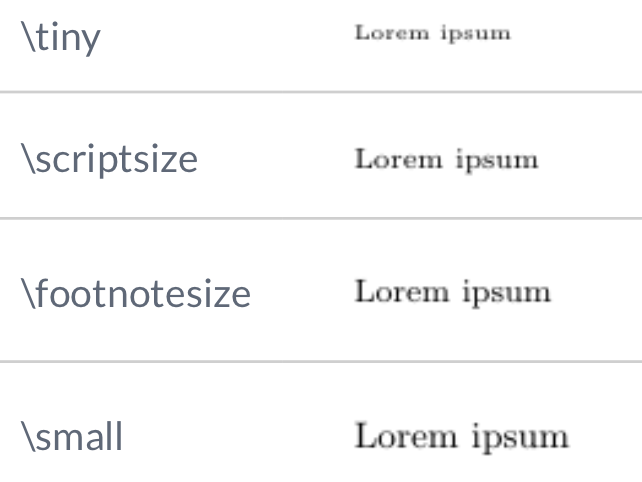
\includegraphics[width=0.5\linewidth]{figures/sample-content/latex_font_sizes} 

}

\caption{Font sizes in LaTeX}\label{fig:latex-font-sizing}
\end{figure}

You could use these to manually adjust the font size in your longtable in two steps:

1. Wrap the longtable environment in, e.g., a `scriptsize` environment, by doing a string replacement in the output from `kable`/`kableExtra`
2. Add the attributes that make R Markdown understand that the table is a table (it seems R drops these when we do the string replacement)


\begin{scriptsize}
\begin{longtable}{lrrrrrrrrrrr}
\toprule
  & mpg & cyl & disp & hp & drat & wt & qsec & vs & am & gear & carb\\
\midrule
\endfirsthead
\multicolumn{12}{@{}l}{\textit{(continued)}}\\
\toprule
  & mpg & cyl & disp & hp & drat & wt & qsec & vs & am & gear & carb\\
\midrule
\endhead

\endfoot
\bottomrule
\endlastfoot
Mazda RX4 & 21.0 & 6 & 160.0 & 110 & 3.90 & 2.620 & 16.46 & 0 & 1 & 4 & 4\\
Mazda RX4 Wag & 21.0 & 6 & 160.0 & 110 & 3.90 & 2.875 & 17.02 & 0 & 1 & 4 & 4\\
Datsun 710 & 22.8 & 4 & 108.0 & 93 & 3.85 & 2.320 & 18.61 & 1 & 1 & 4 & 1\\
Hornet 4 Drive & 21.4 & 6 & 258.0 & 110 & 3.08 & 3.215 & 19.44 & 1 & 0 & 3 & 1\\
Hornet Sportabout & 18.7 & 8 & 360.0 & 175 & 3.15 & 3.440 & 17.02 & 0 & 0 & 3 & 2\\
\addlinespace
Valiant & 18.1 & 6 & 225.0 & 105 & 2.76 & 3.460 & 20.22 & 1 & 0 & 3 & 1\\
Duster 360 & 14.3 & 8 & 360.0 & 245 & 3.21 & 3.570 & 15.84 & 0 & 0 & 3 & 4\\
Merc 240D & 24.4 & 4 & 146.7 & 62 & 3.69 & 3.190 & 20.00 & 1 & 0 & 4 & 2\\
Merc 230 & 22.8 & 4 & 140.8 & 95 & 3.92 & 3.150 & 22.90 & 1 & 0 & 4 & 2\\
Merc 280 & 19.2 & 6 & 167.6 & 123 & 3.92 & 3.440 & 18.30 & 1 & 0 & 4 & 4\\
\addlinespace
Merc 280C & 17.8 & 6 & 167.6 & 123 & 3.92 & 3.440 & 18.90 & 1 & 0 & 4 & 4\\
Merc 450SE & 16.4 & 8 & 275.8 & 180 & 3.07 & 4.070 & 17.40 & 0 & 0 & 3 & 3\\
Merc 450SL & 17.3 & 8 & 275.8 & 180 & 3.07 & 3.730 & 17.60 & 0 & 0 & 3 & 3\\
Merc 450SLC & 15.2 & 8 & 275.8 & 180 & 3.07 & 3.780 & 18.00 & 0 & 0 & 3 & 3\\
Cadillac Fleetwood & 10.4 & 8 & 472.0 & 205 & 2.93 & 5.250 & 17.98 & 0 & 0 & 3 & 4\\
\addlinespace
Lincoln Continental & 10.4 & 8 & 460.0 & 215 & 3.00 & 5.424 & 17.82 & 0 & 0 & 3 & 4\\
Chrysler Imperial & 14.7 & 8 & 440.0 & 230 & 3.23 & 5.345 & 17.42 & 0 & 0 & 3 & 4\\
Fiat 128 & 32.4 & 4 & 78.7 & 66 & 4.08 & 2.200 & 19.47 & 1 & 1 & 4 & 1\\
Honda Civic & 30.4 & 4 & 75.7 & 52 & 4.93 & 1.615 & 18.52 & 1 & 1 & 4 & 2\\
Toyota Corolla & 33.9 & 4 & 71.1 & 65 & 4.22 & 1.835 & 19.90 & 1 & 1 & 4 & 1\\
\addlinespace
Toyota Corona & 21.5 & 4 & 120.1 & 97 & 3.70 & 2.465 & 20.01 & 1 & 0 & 3 & 1\\
Dodge Challenger & 15.5 & 8 & 318.0 & 150 & 2.76 & 3.520 & 16.87 & 0 & 0 & 3 & 2\\
AMC Javelin & 15.2 & 8 & 304.0 & 150 & 3.15 & 3.435 & 17.30 & 0 & 0 & 3 & 2\\
Camaro Z28 & 13.3 & 8 & 350.0 & 245 & 3.73 & 3.840 & 15.41 & 0 & 0 & 3 & 4\\
Pontiac Firebird & 19.2 & 8 & 400.0 & 175 & 3.08 & 3.845 & 17.05 & 0 & 0 & 3 & 2\\
\addlinespace
Fiat X1-9 & 27.3 & 4 & 79.0 & 66 & 4.08 & 1.935 & 18.90 & 1 & 1 & 4 & 1\\
Porsche 914-2 & 26.0 & 4 & 120.3 & 91 & 4.43 & 2.140 & 16.70 & 0 & 1 & 5 & 2\\
Lotus Europa & 30.4 & 4 & 95.1 & 113 & 3.77 & 1.513 & 16.90 & 1 & 1 & 5 & 2\\
Ford Pantera L & 15.8 & 8 & 351.0 & 264 & 4.22 & 3.170 & 14.50 & 0 & 1 & 5 & 4\\
Ferrari Dino & 19.7 & 6 & 145.0 & 175 & 3.62 & 2.770 & 15.50 & 0 & 1 & 5 & 6\\
\addlinespace
Maserati Bora & 15.0 & 8 & 301.0 & 335 & 3.54 & 3.570 & 14.60 & 0 & 1 & 5 & 8\\
Volvo 142E & 21.4 & 4 & 121.0 & 109 & 4.11 & 2.780 & 18.60 & 1 & 1 & 4 & 2\\
Mazda RX41 & 21.0 & 6 & 160.0 & 110 & 3.90 & 2.620 & 16.46 & 0 & 1 & 4 & 4\\
Mazda RX4 Wag1 & 21.0 & 6 & 160.0 & 110 & 3.90 & 2.875 & 17.02 & 0 & 1 & 4 & 4\\
Datsun 7101 & 22.8 & 4 & 108.0 & 93 & 3.85 & 2.320 & 18.61 & 1 & 1 & 4 & 1\\
\addlinespace
Hornet 4 Drive1 & 21.4 & 6 & 258.0 & 110 & 3.08 & 3.215 & 19.44 & 1 & 0 & 3 & 1\\
Hornet Sportabout1 & 18.7 & 8 & 360.0 & 175 & 3.15 & 3.440 & 17.02 & 0 & 0 & 3 & 2\\
Valiant1 & 18.1 & 6 & 225.0 & 105 & 2.76 & 3.460 & 20.22 & 1 & 0 & 3 & 1\\
Duster 3601 & 14.3 & 8 & 360.0 & 245 & 3.21 & 3.570 & 15.84 & 0 & 0 & 3 & 4\\
Merc 240D1 & 24.4 & 4 & 146.7 & 62 & 3.69 & 3.190 & 20.00 & 1 & 0 & 4 & 2\\
\addlinespace
Merc 2301 & 22.8 & 4 & 140.8 & 95 & 3.92 & 3.150 & 22.90 & 1 & 0 & 4 & 2\\
Merc 2801 & 19.2 & 6 & 167.6 & 123 & 3.92 & 3.440 & 18.30 & 1 & 0 & 4 & 4\\
Merc 280C1 & 17.8 & 6 & 167.6 & 123 & 3.92 & 3.440 & 18.90 & 1 & 0 & 4 & 4\\
Merc 450SE1 & 16.4 & 8 & 275.8 & 180 & 3.07 & 4.070 & 17.40 & 0 & 0 & 3 & 3\\
Merc 450SL1 & 17.3 & 8 & 275.8 & 180 & 3.07 & 3.730 & 17.60 & 0 & 0 & 3 & 3\\
\addlinespace
Merc 450SLC1 & 15.2 & 8 & 275.8 & 180 & 3.07 & 3.780 & 18.00 & 0 & 0 & 3 & 3\\
Cadillac Fleetwood1 & 10.4 & 8 & 472.0 & 205 & 2.93 & 5.250 & 17.98 & 0 & 0 & 3 & 4\\
Lincoln Continental1 & 10.4 & 8 & 460.0 & 215 & 3.00 & 5.424 & 17.82 & 0 & 0 & 3 & 4\\
Chrysler Imperial1 & 14.7 & 8 & 440.0 & 230 & 3.23 & 5.345 & 17.42 & 0 & 0 & 3 & 4\\
Fiat 1281 & 32.4 & 4 & 78.7 & 66 & 4.08 & 2.200 & 19.47 & 1 & 1 & 4 & 1\\
\addlinespace
Honda Civic1 & 30.4 & 4 & 75.7 & 52 & 4.93 & 1.615 & 18.52 & 1 & 1 & 4 & 2\\
Toyota Corolla1 & 33.9 & 4 & 71.1 & 65 & 4.22 & 1.835 & 19.90 & 1 & 1 & 4 & 1\\
Toyota Corona1 & 21.5 & 4 & 120.1 & 97 & 3.70 & 2.465 & 20.01 & 1 & 0 & 3 & 1\\
Dodge Challenger1 & 15.5 & 8 & 318.0 & 150 & 2.76 & 3.520 & 16.87 & 0 & 0 & 3 & 2\\
AMC Javelin1 & 15.2 & 8 & 304.0 & 150 & 3.15 & 3.435 & 17.30 & 0 & 0 & 3 & 2\\
\addlinespace
Camaro Z281 & 13.3 & 8 & 350.0 & 245 & 3.73 & 3.840 & 15.41 & 0 & 0 & 3 & 4\\
Pontiac Firebird1 & 19.2 & 8 & 400.0 & 175 & 3.08 & 3.845 & 17.05 & 0 & 0 & 3 & 2\\
Fiat X1-91 & 27.3 & 4 & 79.0 & 66 & 4.08 & 1.935 & 18.90 & 1 & 1 & 4 & 1\\
Porsche 914-21 & 26.0 & 4 & 120.3 & 91 & 4.43 & 2.140 & 16.70 & 0 & 1 & 5 & 2\\
Lotus Europa1 & 30.4 & 4 & 95.1 & 113 & 3.77 & 1.513 & 16.90 & 1 & 1 & 5 & 2\\
\addlinespace
Ford Pantera L1 & 15.8 & 8 & 351.0 & 264 & 4.22 & 3.170 & 14.50 & 0 & 1 & 5 & 4\\
Ferrari Dino1 & 19.7 & 6 & 145.0 & 175 & 3.62 & 2.770 & 15.50 & 0 & 1 & 5 & 6\\
Maserati Bora1 & 15.0 & 8 & 301.0 & 335 & 3.54 & 3.570 & 14.60 & 0 & 1 & 5 & 8\\
Volvo 142E1 & 21.4 & 4 & 121.0 & 109 & 4.11 & 2.780 & 18.60 & 1 & 1 & 4 & 2\\*
\end{longtable}
\end{scriptsize}

<!--chapter:end:04-Discussion.Rmd-->

output:
  #bookdown::html_document2: default
  #bookdown::word_document2: default
  bookdown::pdf_document2: 
    template: templates/template.tex
documentclass: book
#bibliography: [bibliography/references.bib, bibliography/additional-references.bib]
---






# Training Event Results {#cites-and-refs}

\chaptermark{Citations and cross-refs}
\minitoc <!-- this will include a mini table of contents-->


## CEPEH Training Event C1


The CEPEH training event C1 held at the premises of University of Nottingham aiming to prepare participants for the practical elements of co-creation and implementation of chatbots as an educational resource. It combined both theoretical and hands-on training.
15 participants were from RISE, AUTH, UoN.

Project managers of partners signposted the person involved, and relevant announcements were made though social media channels to the wider public. External to the project speakers were from University of Leeds, and Computer Science Department of University of Nottingham. It included academics, medical doctors, and researchers with focus both on clinical research and digital innovations in healthcare education and IT specialist/learning technologists 11.18 years of experiences (SD=7.2). A balance between male and female participants achieved.



 
# Overall Training Events Evalaution


Participants were asked to highlight what they liked for each day and how each day can be improved. Findings are described below per day of the training event


Day 1  
The participants comment that they liked the design method for educational resources presented using a co-creation approach, they liked the interactions with other groups, and they liked the overview of existing chatbot resources of the partners. On the areas that can be improved, more media material were requested.


Day 2
Participants enjoyed the presentation from the invited speaker from another faculty of the University of Nottingham, the CEPEH recources presented and the storyboarding process. Participants highlighted that the participation of more clinicians in the event would be an added value in regards with the storyboarding process.


Day3
Participants liked the hands-on activities of the day also enjoyed the creativity of the groups on the online chatbot development tool. As an area of improvement, participants wanted more time on hands on sections.










## CEPEH Training Event 2

**Pre-Training Event survey May 9th-13th 2022 Thessaloniki, Greece**

Twenty-six participants attended the Training Event, along with approximately 10 staff members. There were 21 undergraduate students and 5 postgraduate students, who completed the survey for a total of 26 responses. There were 86% of participants who stated they had not been to a similar event like the training event CEPEH facilitated. There were 90% of students who found the event schedule very organised, and 70% agreed most of the planned sessions were relevant to that interest with the remaining 30% not having enough experience to understand the context to determine if they are interested in the training event. There were 95% of students agreeing or strongly agreeing the training event location is great, the remaining person did not leave additional comments. 


Table 1 suggested attendees had minimal intention to share their own ideas due to lack of previous experience of attending such events, or due to lack of knowledge on the area. However, most were interested in listening to other groups and hearing contextual cases in healthcare.



There were 77% of participants stated they were novices in experience with chatbots in healthcare and were attending to learn more.  The remaining 23% (7 students) stated they were competent and had limited experience with chatbots in healthcare.


One day had several events regarding cybersecurity in healthcare. When asked before these events, 83% stated they were neutral or disagreed that they felt confident about their cybersecurity knowledge in healthcare. In addition, 80% stated they when neutral or disagreed that they felt they had strong cybersecurity safety in healthcare.  Table 2 shows the main pre and post results suggesting a positive experience for more than 75% of attendees on all measures. 



There were 90% (23) of students who heard about the event through a lecturer or a professor, the CEPEH newsletter (2), and 1 person was informed through the anatomy tutoring system at Karolinska Institute. Additionally, 60% suggested the training event to somebody else before the course started.


There were six individuals who stated neutral or disagree when asked if having issues on registration or finding the information for the event. This may have been due to being dependent on emails to receive the information, instead of a dedicated website where the information is available anytime. 


As this was face-to-face, participants were asked about sufficient Covid-19 precautions in place at the facility, 94% agreed with sufficient precautions, two individuals stated no but did not give further information in the additional input box provided.
In summary, most participants were undergraduate students with novice experience, happy with the training event location, felt the sessions were relevant to them, and most shared the event with their colleagues. The values of co-creation, chatbots in healthcare, and taking patient history were bestowed to students in an engaging and well-received manner. Notably, the highest ratings were for staff friendliness which is key to engagement and consistent interaction throughout the intense and long 5-day duration. The sessions were recorded there for the online recordings may be viewed with higher numbers over the subsequent weeks. 



The usual way to include citations in an *R Markdown* document is to put references in a plain text file with the extension **.bib**, in **BibTex** format.[^bib-formats]
Then reference the path to this file in **index.Rmd**'s YAML header with `bibliography: example.bib`.

[^bib-formats]: The bibliography can be in other formats as well, including EndNote (**.enl**) and RIS (**.ris**), see [rmarkdown.rstudio.com/authoring_bibliographies_and_citations](https://rmarkdown.rstudio.com/authoring_bibliographies_and_citations.html).

Most reference managers can create a .bib file with you references automatically.
However, the **by far** best reference manager to use with *R Markdown* is [Zotero](https://www.zotero.org) with the [Better BibTex plug-in](https://retorque.re/zotero-better-bibtex/), because the `citr` plugin for RStudio (see below) can read references directly from your Zotero library!

Here is an example of an entry in a **.bib** file:
```bibtex
@article{Shea2014,
  author =        {Shea, Nicholas and Boldt, Annika},
  journal =       {Trends in Cognitive Sciences},
  pages =         {186--193},
  title =         {{Supra-personal cognitive control}},
  volume =        {18},
  year =          {2014},
  doi =           {10.1016/j.tics.2014.01.006},
}
\end{verbatim}

In this entry highlighted section, `Shea2014' is the \textbf{citation identifier}.
To default way to cite an entry in your text is with this syntax: \texttt{{[}@citation-identifier{]}}.

So I might cite some things (\protect\hyperlink{ref-Lottridge2012}{Lottridge et al., 2012}; \protect\hyperlink{ref-Mill1965}{Mill, 1965 {[}1843{]}}; \protect\hyperlink{ref-Shea2014}{Shea et al., 2014}).

\hypertarget{citation-appearance}{%
\subsection{Appearance of citations and references section (pandoc)}\label{citation-appearance}}

By default, \texttt{oxforddown} lets \href{https://pandoc.org}{Pandoc} handle how citations are inserted in your text and the references section.
You can change the appearance of citations and references by specifying a CSL (Citation Style Language) file in the \texttt{csl} metadata field of \textbf{index.Rmd}.
By default, \texttt{oxforddown} by the Americal Psychological Association (7th Edition), which is an author-year format.

With this style, a number of variations on the citation syntax are useful to know:

\begin{itemize}
\tightlist
\item
  Put author names outside the parenthesis

  \begin{itemize}
  \tightlist
  \item
    This: \texttt{@Shea2014\ says\ blah.}
  \item
    Becomes: Shea et al. (\protect\hyperlink{ref-Shea2014}{2014}) says blah.
  \end{itemize}
\item
  Include only the citation-year (in parenthesis)

  \begin{itemize}
  \tightlist
  \item
    This: \texttt{Shea\ et\ al.\ says\ blah\ {[}-@Shea2014{]}}
  \item
    Becomes: Shea et al.~says blah (\protect\hyperlink{ref-Shea2014}{2014})
  \end{itemize}
\item
  Add text and page or chapter references to the citation

  \begin{itemize}
  \tightlist
  \item
    This: \texttt{{[}see\ @Shea2014,\ pp.\ 33-35;\ also\ @Wu2016,\ ch.\ 1{]}}
  \item
    Becomes: Blah blah (see \protect\hyperlink{ref-Shea2014}{Shea et al., 2014, pp. 33--35}; also \protect\hyperlink{ref-Wu2016}{Wu, 2016}, ch.~1).
  \end{itemize}
\end{itemize}

If you want a numerical citation style instead, try \texttt{csl:\ bibliography/transactions-on-computer-human-interaction.csl} or just have a browse through the \href{https://www.zotero.org/styles}{Zotero Style Repository} and look for one you like.
For convenience, you can set the line spacing and the space between the bibliographic entries in the reference section directly from the YAML header in \textbf{index.Rmd}.

If you prefer to use \texttt{biblatex} or \texttt{natbib} to handle references, see \protect\hyperlink{customising-citations}{this chapter}.

\clearpage

\hypertarget{insert-references-easily-with-rstudios-visual-editor-1}{%
\subsection{Insert references easily with RStudio's Visual Editor}\label{insert-references-easily-with-rstudios-visual-editor-1}}

For an easy way to insert citations, use RStudio's \href{https://rstudio.github.io/visual-markdown-editing/citations.html}{Visual Editor}.
Make sure you have the latest version of RStudio -- the visual editor was originally really buggy, especially in relation to references, but as per v2022.02.0, it's great!

\hypertarget{cross-referencing-1}{%
\section{Cross-referencing}\label{cross-referencing-1}}

We can make cross-references to \textbf{sections} within our document, as well as to \textbf{figures} (images and plots) and \textbf{tables}.

The general cross-referencing syntax is \textbf{\texttt{\textbackslash{}@ref(label)}}

\hypertarget{section-references-1}{%
\subsection{Section references}\label{section-references-1}}

Headers are automatically assigned a reference label, which is the text in lower caps separated by dashes. For example, \texttt{\#\ My\ header} is automatically given the label \texttt{my-header}. So \texttt{\#\ My\ header} can be referenced with \texttt{\textbackslash{}@ref(my-section)}

Remember what we wrote in section \ref{citations}?

We can also use \textbf{hyperlink syntax} and add \# before the label, though this is only guaranteed to work properly in HTML output:

\begin{itemize}
\tightlist
\item
  So if we write \texttt{Remember\ what\ we\ wrote\ up\ in\ {[}the\ previous\ section{]}(\#citations)?}
\item
  It becomes Remember what we wrote up in \protect\hyperlink{citations}{the previous section}?
\end{itemize}

\hypertarget{creating-custom-labels-1}{%
\subsubsection{Creating custom labels}\label{creating-custom-labels-1}}

It is a very good idea to create \textbf{custom labels} for our sections. This is because the automatically assigned labels will change when we change the titles of the sections - to avoid this, we can create the labels ourselves and leave them untouched if we change the section titles.

We create custom labels by adding \texttt{\{\#label\}} after a header, e.g.~\texttt{\#\ My\ section\ \{\#my-label\}}.
See \protect\hyperlink{cites-and-refs}{our chapter title} for an example. That was section \ref{cites-and-refs}.

\hypertarget{figure-image-and-plot-references-1}{%
\subsection{Figure (image and plot) references}\label{figure-image-and-plot-references-1}}

\begin{itemize}
\tightlist
\item
  To refer to figures (i.e.~images and plots) use the syntax \texttt{\textbackslash{}@ref(fig:label)}
\item
  \textbf{GOTCHA}: Figures and tables must have captions if you wish to cross-reference them.
\end{itemize}

Let's add an image:

We refer to this image with \texttt{\textbackslash{}@ref(fig:captain)}.
So Figure \ref{fig:captain} is \protect\hyperlink{fig:captain}{this image}.

And in Figure \ref{fig:cars-plot} we saw a \protect\hyperlink{fig:cars-plot}{cars plot}.

\hypertarget{table-references-1}{%
\subsection{Table references}\label{table-references-1}}

\begin{itemize}
\tightlist
\item
  To refer to tables use the syntax \texttt{\textbackslash{}@ref(tab:label)}
\end{itemize}

Let's include a table:

\begin{table}

\caption{\label{tab:cars-table2}Stopping cars}
\centering
\begin{tabular}[t]{r|r}
\hline
speed & dist\\
\hline
4 & 2\\
\hline
4 & 10\\
\hline
7 & 4\\
\hline
7 & 22\\
\hline
8 & 16\\
\hline
\end{tabular}
\end{table}

We refer to this table with \texttt{\textbackslash{}@ref(tab:cars-table2)}.
So Table \ref{tab:cars-table2} is \protect\hyperlink{tab:cars-table2}{this table}.

And in Table \ref{tab:cars-table} we saw more or less \protect\hyperlink{tab:cars-table}{the same cars table}.

\hypertarget{including-page-numbers}{%
\subsection{Including page numbers}\label{including-page-numbers}}

Finally, in the PDF output we might also want to include the page number of a reference, so that it's easy to find in physical printed output.
LaTeX has a command for this, which looks like this: \texttt{\textbackslash{}pageref\{fig/tab:label\}} (note: curly braces, not parentheses)

When we output to PDF, we can use raw LaTeX directly in our .Rmd files. So if we wanted to include the page of the cars plot we could write:

\begin{itemize}
\tightlist
\item
  This: \texttt{Figure\ \textbackslash{}@ref(fig:cars-plot)\ on\ page\ \textbackslash{}pageref(fig:cars-plot)}
\item
  Becomes: Figure \ref{fig:cars-plot} on page \pageref{fig:cars-plot}
\end{itemize}

\hypertarget{include-page-numbers-only-in-pdf-output}{%
\subsubsection{Include page numbers only in PDF output}\label{include-page-numbers-only-in-pdf-output}}

A problem here is that LaTeX commands don't display in HTML output, so in the gitbook output we'd see simply ``Figure \ref{fig:cars-plot} on page''.

One way to get around this is to use inline R code to insert the text, and use an \texttt{ifelse} statement to check the output format and then insert the appropriate text.

\begin{itemize}
\tightlist
\item
  So this: \texttt{\textasciigrave{}r\ ifelse(knitr::is\_latex\_output(),\ "Figure\ \textbackslash{}\textbackslash{}@ref(fig:cars-plot)\ on\ page\ \textbackslash{}\textbackslash{}pageref\{fig:cars-plot\}",\ "")\textasciigrave{}}
\item
  Inserts this (check this on both PDF and gitbook): Figure \ref{fig:cars-plot} on page \pageref{fig:cars-plot}
\end{itemize}

Note that we need to escape the backslash with another backslash here to get the correct output.

\hypertarget{collaborative-writing}{%
\section{Collaborative writing}\label{collaborative-writing}}

Best practices for collaboration and change tracking when using R Markdown are still an open question.
In the blog post \href{https://livefreeordichotomize.com/2018/09/14/one-year-to-dissertate/}{\textbf{One year to dissertate}} by Lucy D'Agostino, which I highly recommend, the author notes that she knits .Rmd files to a word document, then uses the \texttt{googledrive} R package to send this to Google Drive for comments / revisions from co-authors, then incorporates Google Drive suggestions \emph{by hand} into the .Rmd source files.
This is a bit clunky, and there are ongoing discussions among the \emph{R Markdown} developers about what the best way is to handle collaborative writing (see \href{https://github.com/rstudio/rmarkdown/issues/1463}{issue \#1463} on GitHub, where \href{http://criticmarkup.com}{CriticMarkup} is among the suggestions).

For now, this is an open question in the community of R Markdown users.
I often knit to a format that can easily be imported to Google Docs for comments, then go over suggested revisions and manually incorporate them back in to the .Rmd source files.
For articles, I sometimes upload a near-final draft to \href{https://www.overleaf.com/}{Overleaf}, then collaboratively make final edits to the LaTeX file there.
I suspect some great solution will be developed in the not-to-distant future, probably by the RStudio team.

\hypertarget{additional-resources}{%
\section{Additional resources}\label{additional-resources}}

\begin{itemize}
\item
  \emph{R Markdown: The Definitive Guide} - \url{https://bookdown.org/yihui/rmarkdown/}
\item
  \emph{R for Data Science} - \url{https://r4ds.had.co.nz}
\end{itemize}



\hypertarget{appendix}{%
\chapter*{Appendix}\label{appendix}}
\addcontentsline{toc}{chapter}{Appendix}

\startappendices

\hypertarget{the-first-appendix}{%
\chapter{The First Appendix}\label{the-first-appendix}}

This first appendix includes an R chunk that was hidden in the document (using \texttt{echo\ =\ FALSE}) to help with readibility:

\textbf{In 02-rmd-basics-code.Rmd}

\textbf{And here's another one from the same chapter, i.e.~Chapter \ref{code}:}

\hypertarget{the-second-appendix-for-fun}{%
\chapter{The Second Appendix, for Fun}\label{the-second-appendix-for-fun}}

\hypertarget{references}{%
\chapter*{References}\label{references}}
\addcontentsline{toc}{chapter}{References}

\markboth{References}{}

\hypertarget{refs}{}
\begin{CSLReferences}{1}{0}
\leavevmode\vadjust pre{\hypertarget{ref-von_goethe_wilhelm_1829}{}}%
Goethe, J. W. von. (1829). \emph{Wilhelm {Meisters} {Wanderjahre} oder die {Entsagenden}}. Cotta.

\leavevmode\vadjust pre{\hypertarget{ref-Lottridge2012}{}}%
Lottridge, D., Marschner, E., Wang, E., Romanovsky, M., \& Nass, C. (2012). {Browser design impacts multitasking}. \emph{Proceedings of the Human Factors and Ergonomics Society 56th Annual Meeting}. \url{https://doi.org/10.1177/1071181312561289}

\leavevmode\vadjust pre{\hypertarget{ref-Mill1965}{}}%
Mill, J. S. (1965 {[}1843{]}). \emph{A system of logic, ratiocinative and inductive: Being a connected view of the principles of evidence and the methods of scientific investigation}. Longmans.

\leavevmode\vadjust pre{\hypertarget{ref-Shea2014}{}}%
Shea, N., Boldt, A., Bang, D., Yeung, N., Heyes, C., \& Frith, C. D. (2014). {Supra-personal cognitive control and metacognition}. \emph{Trends in Cognitive Sciences}, \emph{18}(4), 186--193. \url{https://doi.org/10.1016/j.tics.2014.01.006}

\leavevmode\vadjust pre{\hypertarget{ref-Wu2016}{}}%
Wu, T. (2016). \emph{{The Attention Merchants: The Epic Scramble to Get Inside Our Heads}}. Knopf Publishing Group.

\end{CSLReferences}

%%%%% REFERENCES


\end{document}
